\documentclass[twoside]{book}

% Packages required by doxygen
\usepackage{fixltx2e}
\usepackage{calc}
\usepackage{doxygen}
\usepackage[export]{adjustbox} % also loads graphicx
\usepackage{graphicx}
\usepackage[utf8]{inputenc}
\usepackage{makeidx}
\usepackage{multicol}
\usepackage{multirow}
\PassOptionsToPackage{warn}{textcomp}
\usepackage{textcomp}
\usepackage[nointegrals]{wasysym}
\usepackage[table]{xcolor}

% Font selection
\usepackage[T1]{fontenc}
\usepackage[scaled=.90]{helvet}
\usepackage{courier}
\usepackage{amssymb}
\usepackage{sectsty}
\renewcommand{\familydefault}{\sfdefault}
\allsectionsfont{%
  \fontseries{bc}\selectfont%
  \color{darkgray}%
}
\renewcommand{\DoxyLabelFont}{%
  \fontseries{bc}\selectfont%
  \color{darkgray}%
}
\newcommand{\+}{\discretionary{\mbox{\scriptsize$\hookleftarrow$}}{}{}}

% Page & text layout
\usepackage{geometry}
\geometry{%
  a4paper,%
  top=2.5cm,%
  bottom=2.5cm,%
  left=2.5cm,%
  right=2.5cm%
}
\tolerance=750
\hfuzz=15pt
\hbadness=750
\setlength{\emergencystretch}{15pt}
\setlength{\parindent}{0cm}
\setlength{\parskip}{3ex plus 2ex minus 2ex}
\makeatletter
\renewcommand{\paragraph}{%
  \@startsection{paragraph}{4}{0ex}{-1.0ex}{1.0ex}{%
    \normalfont\normalsize\bfseries\SS@parafont%
  }%
}
\renewcommand{\subparagraph}{%
  \@startsection{subparagraph}{5}{0ex}{-1.0ex}{1.0ex}{%
    \normalfont\normalsize\bfseries\SS@subparafont%
  }%
}
\makeatother

% Headers & footers
\usepackage{fancyhdr}
\pagestyle{fancyplain}
\fancyhead[LE]{\fancyplain{}{\bfseries\thepage}}
\fancyhead[CE]{\fancyplain{}{}}
\fancyhead[RE]{\fancyplain{}{\bfseries\leftmark}}
\fancyhead[LO]{\fancyplain{}{\bfseries\rightmark}}
\fancyhead[CO]{\fancyplain{}{}}
\fancyhead[RO]{\fancyplain{}{\bfseries\thepage}}
\fancyfoot[LE]{\fancyplain{}{}}
\fancyfoot[CE]{\fancyplain{}{}}
\fancyfoot[RE]{\fancyplain{}{\bfseries\scriptsize Generated by Doxygen }}
\fancyfoot[LO]{\fancyplain{}{\bfseries\scriptsize Generated by Doxygen }}
\fancyfoot[CO]{\fancyplain{}{}}
\fancyfoot[RO]{\fancyplain{}{}}
\renewcommand{\footrulewidth}{0.4pt}
\renewcommand{\chaptermark}[1]{%
  \markboth{#1}{}%
}
\renewcommand{\sectionmark}[1]{%
  \markright{\thesection\ #1}%
}

% Indices & bibliography
\usepackage{natbib}
\usepackage[titles]{tocloft}
\setcounter{tocdepth}{3}
\setcounter{secnumdepth}{5}
\makeindex

% Hyperlinks (required, but should be loaded last)
\usepackage{ifpdf}
\ifpdf
  \usepackage[pdftex,pagebackref=true]{hyperref}
\else
  \usepackage[ps2pdf,pagebackref=true]{hyperref}
\fi
\hypersetup{%
  colorlinks=true,%
  linkcolor=blue,%
  citecolor=blue,%
  unicode%
}

% Custom commands
\newcommand{\clearemptydoublepage}{%
  \newpage{\pagestyle{empty}\cleardoublepage}%
}

\usepackage{caption}
\captionsetup{labelsep=space,justification=centering,font={bf},singlelinecheck=off,skip=4pt,position=top}

%===== C O N T E N T S =====

\begin{document}

% Titlepage & ToC
\hypersetup{pageanchor=false,
             bookmarksnumbered=true,
             pdfencoding=unicode
            }
\pagenumbering{roman}
\begin{titlepage}
\vspace*{7cm}
\begin{center}%
{\Large My Project }\\
\vspace*{1cm}
{\large Generated by Doxygen 1.8.11}\\
\end{center}
\end{titlepage}
\clearemptydoublepage
\tableofcontents
\clearemptydoublepage
\pagenumbering{arabic}
\hypersetup{pageanchor=true}

%--- Begin generated contents ---
\chapter{The-\/\+Warehouse-\/\+Helper}
\label{md_README}
\hypertarget{md_README}{}
\mbox{[}E\+N\+PM -\/ 808X Final Project \mbox{]} Implementation of a robot that can pickup, transport and dropoff one or more loads between various known logistics stations based on user or system-\/generated orders that are not known a priori.

\href{https://travis-ci.org/Ip-umd/The_Warehouse_Helper}{\tt } \href{https://coveralls.io/github/Ip-umd/The_Warehouse_Helper?branch=iteration1}{\tt } \href{https://opensource.org/licenses/BSD-3-Clause}{\tt }

\subsection*{Project Overview}

We have developed a Warehouse Helper robot for Acme Robotics. The Turtlebot3, which we have used as a base robot, uses a path-\/planning algorithm(\+A$\ast$ algorithm) to navigate in a predefined map of warehouse. It then creates an optimal path from start station to goal station, while avoiding obstacles.

We also have implemented the funtionality that robot can navigate to intermediate stations between start station and goal location.

\subsection*{Authors}

Ishan Patel
\begin{DoxyItemize}
\item Robotics student at University of Maryland
\item Areas of interests are perception and planning of self-\/driving vehicles.
\end{DoxyItemize}

Nakul Patel
\begin{DoxyItemize}
\item Robotics student at University of Maryland
\item Areas of interests are perception and planning of autonomous vehicles.
\end{DoxyItemize}

Sri Manika Makam
\begin{DoxyItemize}
\item Robotics student at University of Maryland
\item Areas of interests are path-\/planning of autonomous vehicles.
\end{DoxyItemize}

\subsection*{Google Sheet for A\+IP\+:}

\href{https://docs.google.com/spreadsheets/d/1t4cP0wDVoSsd_CHPAsWeQVUyKAmTfhGT0WIE1Eti5zc/edit?ts=5dd5b5d7#gid=1860513107}{\tt https\+://docs.\+google.\+com/spreadsheets/d/1t4c\+P0w\+D\+Vo\+Ssd\+\_\+\+C\+H\+P\+As\+We\+Q\+V\+Uy\+K\+Am\+Tfh\+G\+T0\+W\+I\+E1\+Eti5zc/edit?ts=5dd5b5d7\#gid=1860513107}

\subsection*{Sprint Planning Notes\+:}

\href{https://docs.google.com/document/d/1rJrAD-c7H2RfS4iTaWQ11ydM7skeF1xUm2HMC1adbkw/edit?usp=sharing}{\tt https\+://docs.\+google.\+com/document/d/1r\+Jr\+A\+D-\/c7\+H2\+Rf\+S4i\+Ta\+W\+Q11yd\+M7ske\+F1x\+Um2\+H\+M\+C1adbkw/edit?usp=sharing}

\subsection*{Presentation Slides and Demo Video\+:}

\subsection*{Dependencies}

For this project, you require following dependencies\+:


\begin{DoxyItemize}
\item Ubuntu 16.\+04
\item R\+OS kinetic
\item Gazebo 7.\+x
\item Googletest
\item Open\+CV
\item catkin
\item Turtlebot packages
\end{DoxyItemize}

R\+OS can be installed from the \href{https://wiki.ros.org}{\tt https\+://wiki.\+ros.\+org} site. Click on following link \href{https://wiki.ros.org/kinetic/Installation}{\tt here} to navigate to the installation guide for R\+OS.

To install Turtlebot packages, execute following command in terminal\+: 
\begin{DoxyCode}
1 sudo apt-get install ros-kinetic-turtlebot-gazebo ros-kinetic-turtlebot-apps
       ros-kinetic-turtlebot-rviz-launchers
\end{DoxyCode}



\begin{DoxyItemize}
\item To Install Gazebo 7.\+x follow this link \href{http://gazebosim.org/tutorials?tut=install_ubuntu&ver=7.0}{\tt L\+I\+NK}.
\item To Install Open\+CV follow this link \mbox{[}L\+I\+NK\mbox{]}(\href{https://github.com/kyamagu/mexopencv/wiki/Installation-(Linux,-Octave,-OpenCV-3)}{\tt https\+://github.\+com/kyamagu/mexopencv/wiki/\+Installation-\/(\+Linux,-\/\+Octave,-\/\+Open\+C\+V-\/3)}.
\end{DoxyItemize}

\subsection*{License}

B\+SD 3-\/\+Clause License 
\begin{DoxyCode}
1 Copyright (c) 2019, Ishan Patel, Nakul Patel, Sri Manika Makam
2 All rights reserved.
3 
4 Redistribution and use in source and binary forms, with or without
5 modification, are permitted provided that the following conditions are met:
6 
7 1. Redistributions of source code must retain the above copyright notice, this
8    list of conditions and the following disclaimer.
9 
10 2. Redistributions in binary form must reproduce the above copyright notice,
11    this list of conditions and the following disclaimer in the documentation
12    and/or other materials provided with the distribution.
13 
14 3. Neither the name of the copyright holder nor the names of its
15    contributors may be used to endorse or promote products derived from
16    this software without specific prior written permission.
17 
18 THIS SOFTWARE IS PROVIDED BY THE COPYRIGHT HOLDERS AND CONTRIBUTORS "AS IS"
19 AND ANY EXPRESS OR IMPLIED WARRANTIES, INCLUDING, BUT NOT LIMITED TO, THE
20 IMPLIED WARRANTIES OF MERCHANTABILITY AND FITNESS FOR A PARTICULAR PURPOSE ARE
21 DISCLAIMED. IN NO EVENT SHALL THE COPYRIGHT HOLDER OR CONTRIBUTORS BE LIABLE
22 FOR ANY DIRECT, INDIRECT, INCIDENTAL, SPECIAL, EXEMPLARY, OR CONSEQUENTIAL
23 DAMAGES (INCLUDING, BUT NOT LIMITED TO, PROCUREMENT OF SUBSTITUTE GOODS OR
24 SERVICES; LOSS OF USE, DATA, OR PROFITS; OR BUSINESS INTERRUPTION) HOWEVER
25 CAUSED AND ON ANY THEORY OF LIABILITY, WHETHER IN CONTRACT, STRICT LIABILITY,
26 OR TORT (INCLUDING NEGLIGENCE OR OTHERWISE) ARISING IN ANY WAY OUT OF THE USE
27 OF THIS SOFTWARE, EVEN IF ADVISED OF THE POSSIBILITY OF SUCH DAMAGE.
\end{DoxyCode}


\#\# Package installation 
\begin{DoxyCode}
1 $ mkdir -p ~/catkin\_ws/src
2 $ cd ~/catkin\_ws/
3 $ catkin\_make
4 $ source devel/setup.bash
5 $ cd src/
6 $ git clone --recursive https://github.com/Ip-umd/The\_Warehouse\_Helper.git
7 $ cd ..
8 $ catkin\_make
\end{DoxyCode}
 \subsection*{Instructions to run the program (D\+E\+MO)}

To run the program first open a new terminal window and run following commands. 
\begin{DoxyCode}
1 $ rosclean purge
2 $ cd <path to catkin\_ws>
3 $ source devel/setup.bash
4 $ roslaunch The\_Warehouse\_Helper warehouseHelperTest.launch
\end{DoxyCode}
 $>$\mbox{[}N\+O\+TE\+: {\bfseries Make sure to run the source devel/setup.\+bash command evertime you want to run the package} otherwise the launch file won\textquotesingle{}t detect the package. Also you will see {\bfseries warnings} which our package will output, on the screen till gazebo is launched completely\mbox{]}

\subsection*{Instructions to run R\+OS Unit-\/\+Tests}

The tests are written using gtest and rostest. Close all the running processes before executing the commands below to run the rostest.


\begin{DoxyItemize}
\item main.\+cpp
\item A\+Star\+Test.\+cpp
\item Node\+Param\+Test\+Test.\+cpp
\item \hyperlink{_obstacle_map_test_8cpp}{Obstacle\+Map\+Test.\+cpp}
\item warehouse\+Helper\+Test.\+launch
\end{DoxyItemize}

To run the tests, follow these commands\+: In a new terminal, 
\begin{DoxyCode}
1 roslaunch The\_Warehouse\_Helper warehouseHelperTest.launch
\end{DoxyCode}
 This command, will build a executable for tests named publish\+Test, which can be run using rosrun command.

In another terminal\+: 
\begin{DoxyCode}
1 rosrun The\_Warehouse\_Helper warehouseHelper
\end{DoxyCode}


\subsection*{Doxygen Documentation}

Although the repository contains the documentation, if you\textquotesingle{}d still like to generate it then follow the instructions below.

Install doxygen using below commands 
\begin{DoxyCode}
1 sudo apt-get install doxygen
2 sudo apt-get install doxygen-gui
\end{DoxyCode}
 After installation run following command to open the doxywizard wherein you can fill in the details as required and set the source code folder to the repository as well. Create a new folder in the repository and select that as the destination directory. Add paths to include and src folders and then proceed with the default settings and generate the documentation. 
\begin{DoxyCode}
1 doxywizard
\end{DoxyCode}


\subsection*{Working with Eclipse I\+DE}

\subsection*{Installation}

In your Eclipse workspace directory (or create a new one), checkout the repo (and submodules)


\begin{DoxyCode}
1 mkdir -p ~/workspace
2 cd ~/workspace
3 git clone https://github.com/Ip-umd/The\_Warehouse\_Helper.git
\end{DoxyCode}


In your work directory, use cmake to create an Eclipse project for an \mbox{[}out-\/of-\/source build\mbox{]} of The\+\_\+\+Warehouse\+\_\+\+Helper


\begin{DoxyCode}
1 cd ~/workspace
2 mkdir -p The\_Warehouse\_Helper\_Eclipse
3 cd The\_Warehouse\_Helper\_Eclipse
4 cmake -G "Eclipse CDT4 - Unix Makefiles" -D CMAKE\_BUILD\_TYPE=Debug -D CMAKE\_ECLIPSE\_VERSION=4.7.0 -D
       CMAKE\_CXX\_COMPILER\_ARG1=-std=c++14 ../The\_Warehouse\_Helper/
\end{DoxyCode}
 
\chapter{Class Index}
\section{Class List}
Here are the classes, structs, unions and interfaces with brief descriptions\+:\begin{DoxyCompactList}
\item\contentsline{section}{\hyperlink{class_a_star}{A\+Star} \\*\hyperlink{class_a_star}{A\+Star} class Class for the implementation of A$\ast$ algorithm }{\pageref{class_a_star}}{}
\item\contentsline{section}{\hyperlink{class_node_param}{Node\+Param} \\*\hyperlink{class_node_param}{Node\+Param} class Class for the implementation of costs, velocities, angles and coordinates for nodes in A$\ast$ algorithm }{\pageref{class_node_param}}{}
\item\contentsline{section}{\hyperlink{class_obstacle_map}{Obstacle\+Map} \\*\hyperlink{class_obstacle_map}{Obstacle\+Map} class Class for the implementation of obstacle map }{\pageref{class_obstacle_map}}{}
\end{DoxyCompactList}

\chapter{File Index}
\section{File List}
Here is a list of all documented files with brief descriptions\+:\begin{DoxyCompactList}
\item\contentsline{section}{include/\hyperlink{_a_star_8hpp}{A\+Star.\+hpp} \\*Header file for \hyperlink{_a_star_8cpp}{A\+Star.\+cpp} Defines the member variables and functions in \hyperlink{class_a_star}{A\+Star} class }{\pageref{_a_star_8hpp}}{}
\item\contentsline{section}{include/\hyperlink{_node_param_8hpp}{Node\+Param.\+hpp} \\*Header file for Node\+Param.\+cpp Defines the member variables and functions in \hyperlink{class_node_param}{Node\+Param} class }{\pageref{_node_param_8hpp}}{}
\item\contentsline{section}{include/\hyperlink{_obstacle_map_8hpp}{Obstacle\+Map.\+hpp} \\*Header file for \hyperlink{_obstacle_map_8cpp}{Obstacle\+Map.\+cpp} Defines the member variables and functions in \hyperlink{class_obstacle_map}{Obstacle\+Map} class }{\pageref{_obstacle_map_8hpp}}{}
\item\contentsline{section}{src/\hyperlink{_a_star_8cpp}{A\+Star.\+cpp} \\*Implementation of \hyperlink{class_a_star}{A\+Star} class }{\pageref{_a_star_8cpp}}{}
\item\contentsline{section}{src/\hyperlink{_obstacle_map_8cpp}{Obstacle\+Map.\+cpp} \\*Header file for \hyperlink{_obstacle_map_8cpp}{Obstacle\+Map.\+cpp} }{\pageref{_obstacle_map_8cpp}}{}
\item\contentsline{section}{test/\hyperlink{_obstacle_map_test_8cpp}{Obstacle\+Map\+Test.\+cpp} \\*Unit tests for \hyperlink{class_a_star}{A\+Star} class }{\pageref{_obstacle_map_test_8cpp}}{}
\end{DoxyCompactList}

\chapter{Class Documentation}
\hypertarget{class_a_star}{}\section{A\+Star Class Reference}
\label{class_a_star}\index{A\+Star@{A\+Star}}


\hyperlink{class_a_star}{A\+Star} class Class for the implementation of A$\ast$ algorithm.  




{\ttfamily \#include $<$A\+Star.\+hpp$>$}

\subsection*{Public Member Functions}
\begin{DoxyCompactItemize}
\item 
\hyperlink{class_a_star_ab7cfaf9e1662f45f5fdce245d28c4508}{A\+Star} ()
\begin{DoxyCompactList}\small\item\em Default constructor of \hyperlink{class_a_star}{A\+Star} class. \end{DoxyCompactList}\item 
\hyperlink{class_a_star_ab105ea1d89edefbd8723b0f36652f1aa}{A\+Star} (double rpm1\+Val, double rpm2\+Val, double dt\+Val)
\begin{DoxyCompactList}\small\item\em Constructor of \hyperlink{class_a_star}{A\+Star} class. \end{DoxyCompactList}\item 
\hyperlink{class_a_star_ad246668465621db8818bbe3511fa4ae7}{$\sim$\+A\+Star} ()
\begin{DoxyCompactList}\small\item\em Destructor of \hyperlink{class_a_star}{A\+Star} class. \end{DoxyCompactList}\item 
std\+::vector$<$ std\+::vector$<$ std\+::vector$<$ double $>$ $>$ $>$ \hyperlink{class_a_star_a8fce98f22c2687fa0a214faf9090329c}{back\+Track} (std\+::vector$<$ std\+::vector$<$ std\+::vector$<$ double $>$$>$$>$ back\+List)
\begin{DoxyCompactList}\small\item\em backtrack -\/ Function which implements the backtracking \end{DoxyCompactList}\item 
std\+::vector$<$ std\+::vector$<$ double $>$ $>$ \hyperlink{class_a_star_a6c0e58da70d0dd3402d2fd4e4e3feeec}{motion\+Model} ()
\begin{DoxyCompactList}\small\item\em motion\+Model -\/ Function which describes the motion of robot \end{DoxyCompactList}\item 
std\+::vector$<$ std\+::vector$<$ std\+::vector$<$ double $>$ $>$ $>$ \hyperlink{class_a_star_a48912f3be5ce68c45b07d833ff707cbb}{a\+Star} (std\+::vector$<$ double $>$ start\+Point, std\+::vector$<$ double $>$ goal\+Point)
\begin{DoxyCompactList}\small\item\em motion\+Model -\/ Function which implements the A$\ast$ algorithm \end{DoxyCompactList}\item 
void \hyperlink{class_a_star_abd6f71ed1d4456a99bac7cf872ac7838}{ros\+Turtle} (std\+::vector$<$ std\+::vector$<$ std\+::vector$<$ double $>$$>$$>$ ros\+Inputs)
\begin{DoxyCompactList}\small\item\em motion\+Model -\/ Function for publlishing to R\+OS topic \end{DoxyCompactList}\end{DoxyCompactItemize}


\subsection{Detailed Description}
\hyperlink{class_a_star}{A\+Star} class Class for the implementation of A$\ast$ algorithm. 

\subsection{Constructor \& Destructor Documentation}
\index{A\+Star@{A\+Star}!A\+Star@{A\+Star}}
\index{A\+Star@{A\+Star}!A\+Star@{A\+Star}}
\subsubsection[{\texorpdfstring{A\+Star()}{AStar()}}]{\setlength{\rightskip}{0pt plus 5cm}A\+Star\+::\+A\+Star (
\begin{DoxyParamCaption}
{}
\end{DoxyParamCaption}
)}\hypertarget{class_a_star_ab7cfaf9e1662f45f5fdce245d28c4508}{}\label{class_a_star_ab7cfaf9e1662f45f5fdce245d28c4508}


Default constructor of \hyperlink{class_a_star}{A\+Star} class. 


\begin{DoxyParams}{Parameters}
{\em none} & \\
\hline
\end{DoxyParams}
\begin{DoxyReturn}{Returns}
none Initializes rpm1,rpm2 and dt to zero 
\end{DoxyReturn}
\index{A\+Star@{A\+Star}!A\+Star@{A\+Star}}
\index{A\+Star@{A\+Star}!A\+Star@{A\+Star}}
\subsubsection[{\texorpdfstring{A\+Star(double rpm1\+Val, double rpm2\+Val, double dt\+Val)}{AStar(double rpm1Val, double rpm2Val, double dtVal)}}]{\setlength{\rightskip}{0pt plus 5cm}A\+Star\+::\+A\+Star (
\begin{DoxyParamCaption}
\item[{double}]{rpm1\+Val, }
\item[{double}]{rpm2\+Val, }
\item[{double}]{dt\+Val}
\end{DoxyParamCaption}
)}\hypertarget{class_a_star_ab105ea1d89edefbd8723b0f36652f1aa}{}\label{class_a_star_ab105ea1d89edefbd8723b0f36652f1aa}


Constructor of \hyperlink{class_a_star}{A\+Star} class. 


\begin{DoxyParams}{Parameters}
{\em rpm1\+Val} & of type double \\
\hline
{\em rpm2\+Val} & of type double \\
\hline
{\em dt\+Val} & of type double \\
\hline
\end{DoxyParams}
\begin{DoxyReturn}{Returns}
none Initializes rpm1, rpm2 and dt to the values passed to the constructor 
\end{DoxyReturn}
Setting the values of member variables \index{A\+Star@{A\+Star}!````~A\+Star@{$\sim$\+A\+Star}}
\index{````~A\+Star@{$\sim$\+A\+Star}!A\+Star@{A\+Star}}
\subsubsection[{\texorpdfstring{$\sim$\+A\+Star()}{~AStar()}}]{\setlength{\rightskip}{0pt plus 5cm}A\+Star\+::$\sim$\+A\+Star (
\begin{DoxyParamCaption}
{}
\end{DoxyParamCaption}
)}\hypertarget{class_a_star_ad246668465621db8818bbe3511fa4ae7}{}\label{class_a_star_ad246668465621db8818bbe3511fa4ae7}


Destructor of \hyperlink{class_a_star}{A\+Star} class. 


\begin{DoxyParams}{Parameters}
{\em none} & \\
\hline
\end{DoxyParams}
\begin{DoxyReturn}{Returns}
none Destroys class objects 
\end{DoxyReturn}


\subsection{Member Function Documentation}
\index{A\+Star@{A\+Star}!a\+Star@{a\+Star}}
\index{a\+Star@{a\+Star}!A\+Star@{A\+Star}}
\subsubsection[{\texorpdfstring{a\+Star(std\+::vector$<$ double $>$ start\+Point, std\+::vector$<$ double $>$ goal\+Point)}{aStar(std::vector< double > startPoint, std::vector< double > goalPoint)}}]{\setlength{\rightskip}{0pt plus 5cm}{\bf nest\+Vector} A\+Star\+::a\+Star (
\begin{DoxyParamCaption}
\item[{std\+::vector$<$ double $>$}]{start\+Point, }
\item[{std\+::vector$<$ double $>$}]{goal\+Point}
\end{DoxyParamCaption}
)}\hypertarget{class_a_star_a48912f3be5ce68c45b07d833ff707cbb}{}\label{class_a_star_a48912f3be5ce68c45b07d833ff707cbb}


motion\+Model -\/ Function which implements the A$\ast$ algorithm 


\begin{DoxyParams}{Parameters}
{\em start\+Point} & -\/ coordinates of start\+Point \\
\hline
{\em goal\+Point} & -\/ coordinates of goal\+Point \\
\hline
\end{DoxyParams}
\begin{DoxyReturn}{Returns}
velocities and angles of nodes in backtrack list 
\end{DoxyReturn}
defining struct to implement the priority queue

declaring the variables for storing unvisited and visited nodes

defining the start\+Node

defining the end\+Node

setting the radius of robot

Creating cost\+Map for node exploration

storing the node with least cost in current\+Node

removing the node from unvisited

adding the node in visited

defining the threshold for reaching destination

Checking whether the destination is reached

calling the \hyperlink{class_a_star_a6c0e58da70d0dd3402d2fd4e4e3feeec}{motion\+Model()} function

Exploring all the neighbor nodes

setting the member variables of nodes through setters

setting the member variables of nodes through setters

setting the member variables of nodes through setters

setting the member variables of nodes through setters

setting the member variables of nodes through setters

setting the member variables of nodes through setters

checking if the explored node is within boundaries

checking if the explored node is not hitting the obstacle

updating the cost\+Map

Adding the explored node to unvisited \index{A\+Star@{A\+Star}!back\+Track@{back\+Track}}
\index{back\+Track@{back\+Track}!A\+Star@{A\+Star}}
\subsubsection[{\texorpdfstring{back\+Track(std\+::vector$<$ std\+::vector$<$ std\+::vector$<$ double $>$$>$$>$ back\+List)}{backTrack(std::vector< std::vector< std::vector< double >>> backList)}}]{\setlength{\rightskip}{0pt plus 5cm}{\bf nest\+Vector} A\+Star\+::back\+Track (
\begin{DoxyParamCaption}
\item[{std\+::vector$<$ std\+::vector$<$ std\+::vector$<$ double $>$$>$$>$}]{back\+List}
\end{DoxyParamCaption}
)}\hypertarget{class_a_star_a8fce98f22c2687fa0a214faf9090329c}{}\label{class_a_star_a8fce98f22c2687fa0a214faf9090329c}


backtrack -\/ Function which implements the backtracking 


\begin{DoxyParams}{Parameters}
{\em back\+List} & -\/ contains current\+Node, parent\+Node, velocity and angle for nodes \\
\hline
\end{DoxyParams}
\begin{DoxyReturn}{Returns}
velocity and angles for nodes in the obtained path 
\end{DoxyReturn}
storing the current\+Pos of node

appending velocity and angle

getting the parent from back\+List

checking if parent found

appending velocity and angle in ros\+Inputs

reversing the data stored in path and ros\+Inputs \index{A\+Star@{A\+Star}!motion\+Model@{motion\+Model}}
\index{motion\+Model@{motion\+Model}!A\+Star@{A\+Star}}
\subsubsection[{\texorpdfstring{motion\+Model()}{motionModel()}}]{\setlength{\rightskip}{0pt plus 5cm}std\+::vector$<$ std\+::vector$<$ double $>$ $>$ A\+Star\+::motion\+Model (
\begin{DoxyParamCaption}
{}
\end{DoxyParamCaption}
)}\hypertarget{class_a_star_a6c0e58da70d0dd3402d2fd4e4e3feeec}{}\label{class_a_star_a6c0e58da70d0dd3402d2fd4e4e3feeec}


motion\+Model -\/ Function which describes the motion of robot 


\begin{DoxyParams}{Parameters}
{\em none} & \\
\hline
\end{DoxyParams}
\begin{DoxyReturn}{Returns}
std\+::vector$<$std\+::vector$<$double$>$$>$ -\/ action states for a node 
\end{DoxyReturn}
defining the distance between wheels of Turtlebot3

defining the radius of wheels of Turtlebot3

8 possible action states for a node based on rpm\textquotesingle{}s

defining ur, ul and thetadot based on differential drive model

calculating change in angle

setting the dx for node

setting the dy for node

setting the cost

setting velocity magnitude \index{A\+Star@{A\+Star}!ros\+Turtle@{ros\+Turtle}}
\index{ros\+Turtle@{ros\+Turtle}!A\+Star@{A\+Star}}
\subsubsection[{\texorpdfstring{ros\+Turtle(std\+::vector$<$ std\+::vector$<$ std\+::vector$<$ double $>$$>$$>$ ros\+Inputs)}{rosTurtle(std::vector< std::vector< std::vector< double >>> rosInputs)}}]{\setlength{\rightskip}{0pt plus 5cm}void A\+Star\+::ros\+Turtle (
\begin{DoxyParamCaption}
\item[{std\+::vector$<$ std\+::vector$<$ std\+::vector$<$ double $>$$>$$>$}]{ros\+Inputs}
\end{DoxyParamCaption}
)}\hypertarget{class_a_star_abd6f71ed1d4456a99bac7cf872ac7838}{}\label{class_a_star_abd6f71ed1d4456a99bac7cf872ac7838}


motion\+Model -\/ Function for publlishing to R\+OS topic 


\begin{DoxyParams}{Parameters}
{\em ros\+Inputs} & -\/ variable having velocities and angles from back\+Track function \\
\hline
\end{DoxyParams}
\begin{DoxyReturn}{Returns}
none
\end{DoxyReturn}
This function creates a R\+OS node, which publishes the velocities and angles to the cmd\+\_\+vel topic, which Turtlebot uses to navigate on the path returned by A$\ast$ algorithm Defining the publisher for cmd\+\_\+vel topic

Declaring the object of geometry\+\_\+msgs\+::\+Twist

setting the publishing rate to 10\+HZ

stop the robot if goal is reached

Setting the linear and angular velocities

Publishing the msg on topic 

The documentation for this class was generated from the following files\+:\begin{DoxyCompactItemize}
\item 
include/\hyperlink{_a_star_8hpp}{A\+Star.\+hpp}\item 
src/\hyperlink{_a_star_8cpp}{A\+Star.\+cpp}\end{DoxyCompactItemize}

\hypertarget{class_node_param}{}\section{Node\+Param Class Reference}
\label{class_node_param}\index{Node\+Param@{Node\+Param}}


\hyperlink{class_node_param}{Node\+Param} class Class for the implementation of costs, velocities, angles and coordinates for nodes in A$\ast$ algorithm.  




{\ttfamily \#include $<$Node\+Param.\+hpp$>$}

\subsection*{Public Member Functions}
\begin{DoxyCompactItemize}
\item 
\hyperlink{class_node_param_a4f80268d34f5c0811db92e45cea28163}{Node\+Param} ()
\begin{DoxyCompactList}\small\item\em Default constructor of Node\+Paramclass. \end{DoxyCompactList}\item 
\hyperlink{class_node_param_ad6eeee163bee98665a25d223e2bb807d}{$\sim$\+Node\+Param} ()
\begin{DoxyCompactList}\small\item\em Destructor of \hyperlink{class_node_param}{Node\+Param} class. \end{DoxyCompactList}\item 
std\+::vector$<$ double $>$ \hyperlink{class_node_param_aedda6fd37a4341d1d2be03e962707e4e}{get\+Current} ()
\begin{DoxyCompactList}\small\item\em get\+Current function \end{DoxyCompactList}\item 
void \hyperlink{class_node_param_a72ef1f23b16ccf9eb0e266123d147718}{set\+Current} (std\+::vector$<$ double $>$ current)
\begin{DoxyCompactList}\small\item\em set\+Current function \end{DoxyCompactList}\item 
std\+::vector$<$ double $>$ \hyperlink{class_node_param_a6f06db02196c42fd3aab6101f3f90500}{get\+Parent} ()
\begin{DoxyCompactList}\small\item\em get\+Parent function \end{DoxyCompactList}\item 
void \hyperlink{class_node_param_ad460d4b4ef9d9225ce6f5c8c69b6d1f5}{set\+Parent} (std\+::vector$<$ double $>$ parent)
\begin{DoxyCompactList}\small\item\em set\+Parent function \end{DoxyCompactList}\item 
double \hyperlink{class_node_param_a46aa96e914b2971aa0f2fb9f497bea83}{get\+G\+Cost} ()
\begin{DoxyCompactList}\small\item\em get\+G\+Cost function \end{DoxyCompactList}\item 
void \hyperlink{class_node_param_a75706108ff639d3bf82f264a4dd63de1}{set\+G\+Cost} (double cost\+To\+Go)
\begin{DoxyCompactList}\small\item\em set\+G\+Cost function \end{DoxyCompactList}\item 
double \hyperlink{class_node_param_a052abd98278508034916473f16abd90f}{get\+H\+Cost} ()
\begin{DoxyCompactList}\small\item\em get\+H\+Cost function \end{DoxyCompactList}\item 
void \hyperlink{class_node_param_abdceff8539f713c871b14e0c22b2d7ee}{set\+H\+Cost} (double cost\+To\+Come)
\begin{DoxyCompactList}\small\item\em set\+H\+Cost function \end{DoxyCompactList}\item 
double \hyperlink{class_node_param_a721f207737bd94b350344895a48a9c31}{get\+Total\+Cost} ()
\begin{DoxyCompactList}\small\item\em get\+Total\+Cost function \end{DoxyCompactList}\item 
void \hyperlink{class_node_param_aba159470af0fa4397b29bddfbadbf671}{set\+Total\+Cost} (double total)
\begin{DoxyCompactList}\small\item\em set\+Total\+Cost function \end{DoxyCompactList}\item 
double \hyperlink{class_node_param_af5699295aa1d1bd23c91d7c7504bef32}{get\+Theta} ()
\begin{DoxyCompactList}\small\item\em get\+Theta function \end{DoxyCompactList}\item 
void \hyperlink{class_node_param_ae72c374809beb88a2ac395584135d009}{set\+Theta} (double th)
\begin{DoxyCompactList}\small\item\em set\+Theta function \end{DoxyCompactList}\item 
double \hyperlink{class_node_param_a9ae847d012e6a33d390eb468cb5c3e83}{get\+D\+Theta} ()
\begin{DoxyCompactList}\small\item\em get\+D\+Theta function \end{DoxyCompactList}\item 
void \hyperlink{class_node_param_a501fb82083ddc6b2c3edd84694cc0bae}{set\+D\+Theta} (double dth)
\begin{DoxyCompactList}\small\item\em set\+D\+Theta function \end{DoxyCompactList}\item 
double \hyperlink{class_node_param_a2c1d2ef1833a0c4697d1a3a8c21a29e0}{get\+Dx} ()
\begin{DoxyCompactList}\small\item\em get\+Dx function \end{DoxyCompactList}\item 
void \hyperlink{class_node_param_a9842fb657d570474338bf798cd9851b4}{set\+Dx} (double dX)
\begin{DoxyCompactList}\small\item\em set\+Dx function \end{DoxyCompactList}\item 
double \hyperlink{class_node_param_ace7de13cf60fa1037d8891e9ab484587}{get\+Dy} ()
\begin{DoxyCompactList}\small\item\em get\+Dy function \end{DoxyCompactList}\item 
void \hyperlink{class_node_param_a15ae6e0cab9b1b72e20d4c7bafc19de8}{set\+Dy} (double dY)
\begin{DoxyCompactList}\small\item\em set\+Dy function \end{DoxyCompactList}\end{DoxyCompactItemize}


\subsection{Detailed Description}
\hyperlink{class_node_param}{Node\+Param} class Class for the implementation of costs, velocities, angles and coordinates for nodes in A$\ast$ algorithm. 

\subsection{Constructor \& Destructor Documentation}
\index{Node\+Param@{Node\+Param}!Node\+Param@{Node\+Param}}
\index{Node\+Param@{Node\+Param}!Node\+Param@{Node\+Param}}
\subsubsection[{\texorpdfstring{Node\+Param()}{NodeParam()}}]{\setlength{\rightskip}{0pt plus 5cm}Node\+Param\+::\+Node\+Param (
\begin{DoxyParamCaption}
{}
\end{DoxyParamCaption}
)}\hypertarget{class_node_param_a4f80268d34f5c0811db92e45cea28163}{}\label{class_node_param_a4f80268d34f5c0811db92e45cea28163}


Default constructor of Node\+Paramclass. 


\begin{DoxyParams}{Parameters}
{\em none} & \\
\hline
\end{DoxyParams}
\begin{DoxyReturn}{Returns}
none Initializes all the private data members of the class to zero 
\end{DoxyReturn}
\index{Node\+Param@{Node\+Param}!````~Node\+Param@{$\sim$\+Node\+Param}}
\index{````~Node\+Param@{$\sim$\+Node\+Param}!Node\+Param@{Node\+Param}}
\subsubsection[{\texorpdfstring{$\sim$\+Node\+Param()}{~NodeParam()}}]{\setlength{\rightskip}{0pt plus 5cm}Node\+Param\+::$\sim$\+Node\+Param (
\begin{DoxyParamCaption}
{}
\end{DoxyParamCaption}
)}\hypertarget{class_node_param_ad6eeee163bee98665a25d223e2bb807d}{}\label{class_node_param_ad6eeee163bee98665a25d223e2bb807d}


Destructor of \hyperlink{class_node_param}{Node\+Param} class. 


\begin{DoxyParams}{Parameters}
{\em none} & \\
\hline
\end{DoxyParams}
\begin{DoxyReturn}{Returns}
none Destroys class objects 
\end{DoxyReturn}


\subsection{Member Function Documentation}
\index{Node\+Param@{Node\+Param}!get\+Current@{get\+Current}}
\index{get\+Current@{get\+Current}!Node\+Param@{Node\+Param}}
\subsubsection[{\texorpdfstring{get\+Current()}{getCurrent()}}]{\setlength{\rightskip}{0pt plus 5cm}std\+::vector$<$ double $>$ Node\+Param\+::get\+Current (
\begin{DoxyParamCaption}
{}
\end{DoxyParamCaption}
)}\hypertarget{class_node_param_aedda6fd37a4341d1d2be03e962707e4e}{}\label{class_node_param_aedda6fd37a4341d1d2be03e962707e4e}


get\+Current function 


\begin{DoxyParams}{Parameters}
{\em none} & \\
\hline
\end{DoxyParams}
\begin{DoxyReturn}{Returns}
std\+::vector$<$double$>$ -\/ current\+Node Returns the current\+Node upon request 
\end{DoxyReturn}
returns current\+Node \index{Node\+Param@{Node\+Param}!get\+D\+Theta@{get\+D\+Theta}}
\index{get\+D\+Theta@{get\+D\+Theta}!Node\+Param@{Node\+Param}}
\subsubsection[{\texorpdfstring{get\+D\+Theta()}{getDTheta()}}]{\setlength{\rightskip}{0pt plus 5cm}double Node\+Param\+::get\+D\+Theta (
\begin{DoxyParamCaption}
{}
\end{DoxyParamCaption}
)}\hypertarget{class_node_param_a9ae847d012e6a33d390eb468cb5c3e83}{}\label{class_node_param_a9ae847d012e6a33d390eb468cb5c3e83}


get\+D\+Theta function 


\begin{DoxyParams}{Parameters}
{\em none} & \\
\hline
\end{DoxyParams}
\begin{DoxyReturn}{Returns}
double -\/dtheta Returns the dtheta upon request 
\end{DoxyReturn}
returns dtheta \index{Node\+Param@{Node\+Param}!get\+Dx@{get\+Dx}}
\index{get\+Dx@{get\+Dx}!Node\+Param@{Node\+Param}}
\subsubsection[{\texorpdfstring{get\+Dx()}{getDx()}}]{\setlength{\rightskip}{0pt plus 5cm}double Node\+Param\+::get\+Dx (
\begin{DoxyParamCaption}
{}
\end{DoxyParamCaption}
)}\hypertarget{class_node_param_a2c1d2ef1833a0c4697d1a3a8c21a29e0}{}\label{class_node_param_a2c1d2ef1833a0c4697d1a3a8c21a29e0}


get\+Dx function 


\begin{DoxyParams}{Parameters}
{\em none} & \\
\hline
\end{DoxyParams}
\begin{DoxyReturn}{Returns}
double -\/ dx Returns the dx upon request 
\end{DoxyReturn}
returns dx \index{Node\+Param@{Node\+Param}!get\+Dy@{get\+Dy}}
\index{get\+Dy@{get\+Dy}!Node\+Param@{Node\+Param}}
\subsubsection[{\texorpdfstring{get\+Dy()}{getDy()}}]{\setlength{\rightskip}{0pt plus 5cm}double Node\+Param\+::get\+Dy (
\begin{DoxyParamCaption}
{}
\end{DoxyParamCaption}
)}\hypertarget{class_node_param_ace7de13cf60fa1037d8891e9ab484587}{}\label{class_node_param_ace7de13cf60fa1037d8891e9ab484587}


get\+Dy function 


\begin{DoxyParams}{Parameters}
{\em none} & \\
\hline
\end{DoxyParams}
\begin{DoxyReturn}{Returns}
double -\/ dy Returns the dy upon request 
\end{DoxyReturn}
returns dy \index{Node\+Param@{Node\+Param}!get\+G\+Cost@{get\+G\+Cost}}
\index{get\+G\+Cost@{get\+G\+Cost}!Node\+Param@{Node\+Param}}
\subsubsection[{\texorpdfstring{get\+G\+Cost()}{getGCost()}}]{\setlength{\rightskip}{0pt plus 5cm}double Node\+Param\+::get\+G\+Cost (
\begin{DoxyParamCaption}
{}
\end{DoxyParamCaption}
)}\hypertarget{class_node_param_a46aa96e914b2971aa0f2fb9f497bea83}{}\label{class_node_param_a46aa96e914b2971aa0f2fb9f497bea83}


get\+G\+Cost function 


\begin{DoxyParams}{Parameters}
{\em none} & \\
\hline
\end{DoxyParams}
\begin{DoxyReturn}{Returns}
double -\/ g\+Cost Returns the g\+Cost upon request 
\end{DoxyReturn}
returns g\+Cost \index{Node\+Param@{Node\+Param}!get\+H\+Cost@{get\+H\+Cost}}
\index{get\+H\+Cost@{get\+H\+Cost}!Node\+Param@{Node\+Param}}
\subsubsection[{\texorpdfstring{get\+H\+Cost()}{getHCost()}}]{\setlength{\rightskip}{0pt plus 5cm}double Node\+Param\+::get\+H\+Cost (
\begin{DoxyParamCaption}
{}
\end{DoxyParamCaption}
)}\hypertarget{class_node_param_a052abd98278508034916473f16abd90f}{}\label{class_node_param_a052abd98278508034916473f16abd90f}


get\+H\+Cost function 


\begin{DoxyParams}{Parameters}
{\em none} & \\
\hline
\end{DoxyParams}
\begin{DoxyReturn}{Returns}
double -\/ h\+Cost Returns the h\+Cost upon request 
\end{DoxyReturn}
returrns h\+Cost \index{Node\+Param@{Node\+Param}!get\+Parent@{get\+Parent}}
\index{get\+Parent@{get\+Parent}!Node\+Param@{Node\+Param}}
\subsubsection[{\texorpdfstring{get\+Parent()}{getParent()}}]{\setlength{\rightskip}{0pt plus 5cm}std\+::vector$<$ double $>$ Node\+Param\+::get\+Parent (
\begin{DoxyParamCaption}
{}
\end{DoxyParamCaption}
)}\hypertarget{class_node_param_a6f06db02196c42fd3aab6101f3f90500}{}\label{class_node_param_a6f06db02196c42fd3aab6101f3f90500}


get\+Parent function 


\begin{DoxyParams}{Parameters}
{\em none} & \\
\hline
\end{DoxyParams}
\begin{DoxyReturn}{Returns}
std\+::vector$<$double$>$ -\/ parent\+Node Returns the parent\+Node upon request 
\end{DoxyReturn}
returns parent\+Node \index{Node\+Param@{Node\+Param}!get\+Theta@{get\+Theta}}
\index{get\+Theta@{get\+Theta}!Node\+Param@{Node\+Param}}
\subsubsection[{\texorpdfstring{get\+Theta()}{getTheta()}}]{\setlength{\rightskip}{0pt plus 5cm}double Node\+Param\+::get\+Theta (
\begin{DoxyParamCaption}
{}
\end{DoxyParamCaption}
)}\hypertarget{class_node_param_af5699295aa1d1bd23c91d7c7504bef32}{}\label{class_node_param_af5699295aa1d1bd23c91d7c7504bef32}


get\+Theta function 


\begin{DoxyParams}{Parameters}
{\em none} & \\
\hline
\end{DoxyParams}
\begin{DoxyReturn}{Returns}
double -\/ theta Returns the theta upon request 
\end{DoxyReturn}
returns theta \index{Node\+Param@{Node\+Param}!get\+Total\+Cost@{get\+Total\+Cost}}
\index{get\+Total\+Cost@{get\+Total\+Cost}!Node\+Param@{Node\+Param}}
\subsubsection[{\texorpdfstring{get\+Total\+Cost()}{getTotalCost()}}]{\setlength{\rightskip}{0pt plus 5cm}double Node\+Param\+::get\+Total\+Cost (
\begin{DoxyParamCaption}
{}
\end{DoxyParamCaption}
)}\hypertarget{class_node_param_a721f207737bd94b350344895a48a9c31}{}\label{class_node_param_a721f207737bd94b350344895a48a9c31}


get\+Total\+Cost function 


\begin{DoxyParams}{Parameters}
{\em none} & \\
\hline
\end{DoxyParams}
\begin{DoxyReturn}{Returns}
double -\/ total\+Cost Returns the total\+Cost upon request 
\end{DoxyReturn}
returns total\+Cost \index{Node\+Param@{Node\+Param}!set\+Current@{set\+Current}}
\index{set\+Current@{set\+Current}!Node\+Param@{Node\+Param}}
\subsubsection[{\texorpdfstring{set\+Current(std\+::vector$<$ double $>$ current)}{setCurrent(std::vector< double > current)}}]{\setlength{\rightskip}{0pt plus 5cm}void Node\+Param\+::set\+Current (
\begin{DoxyParamCaption}
\item[{std\+::vector$<$ double $>$}]{current}
\end{DoxyParamCaption}
)}\hypertarget{class_node_param_a72ef1f23b16ccf9eb0e266123d147718}{}\label{class_node_param_a72ef1f23b16ccf9eb0e266123d147718}


set\+Current function 


\begin{DoxyParams}{Parameters}
{\em std\+::vector$<$double$>$} & -\/ current \\
\hline
\end{DoxyParams}
\begin{DoxyReturn}{Returns}
none 
\end{DoxyReturn}
setting the value of current\+Node \index{Node\+Param@{Node\+Param}!set\+D\+Theta@{set\+D\+Theta}}
\index{set\+D\+Theta@{set\+D\+Theta}!Node\+Param@{Node\+Param}}
\subsubsection[{\texorpdfstring{set\+D\+Theta(double dth)}{setDTheta(double dth)}}]{\setlength{\rightskip}{0pt plus 5cm}void Node\+Param\+::set\+D\+Theta (
\begin{DoxyParamCaption}
\item[{double}]{dth}
\end{DoxyParamCaption}
)}\hypertarget{class_node_param_a501fb82083ddc6b2c3edd84694cc0bae}{}\label{class_node_param_a501fb82083ddc6b2c3edd84694cc0bae}


set\+D\+Theta function 


\begin{DoxyParams}{Parameters}
{\em double} & -\/ dth \\
\hline
\end{DoxyParams}
\begin{DoxyReturn}{Returns}
none 
\end{DoxyReturn}
sets the value of dtheta \index{Node\+Param@{Node\+Param}!set\+Dx@{set\+Dx}}
\index{set\+Dx@{set\+Dx}!Node\+Param@{Node\+Param}}
\subsubsection[{\texorpdfstring{set\+Dx(double d\+X)}{setDx(double dX)}}]{\setlength{\rightskip}{0pt plus 5cm}void Node\+Param\+::set\+Dx (
\begin{DoxyParamCaption}
\item[{double}]{dX}
\end{DoxyParamCaption}
)}\hypertarget{class_node_param_a9842fb657d570474338bf798cd9851b4}{}\label{class_node_param_a9842fb657d570474338bf798cd9851b4}


set\+Dx function 


\begin{DoxyParams}{Parameters}
{\em double} & -\/ dX \\
\hline
\end{DoxyParams}
\begin{DoxyReturn}{Returns}
none 
\end{DoxyReturn}
sets the value of dx \index{Node\+Param@{Node\+Param}!set\+Dy@{set\+Dy}}
\index{set\+Dy@{set\+Dy}!Node\+Param@{Node\+Param}}
\subsubsection[{\texorpdfstring{set\+Dy(double d\+Y)}{setDy(double dY)}}]{\setlength{\rightskip}{0pt plus 5cm}void Node\+Param\+::set\+Dy (
\begin{DoxyParamCaption}
\item[{double}]{dY}
\end{DoxyParamCaption}
)}\hypertarget{class_node_param_a15ae6e0cab9b1b72e20d4c7bafc19de8}{}\label{class_node_param_a15ae6e0cab9b1b72e20d4c7bafc19de8}


set\+Dy function 


\begin{DoxyParams}{Parameters}
{\em double} & -\/ dY \\
\hline
\end{DoxyParams}
\begin{DoxyReturn}{Returns}
none 
\end{DoxyReturn}
sets the value of dy \index{Node\+Param@{Node\+Param}!set\+G\+Cost@{set\+G\+Cost}}
\index{set\+G\+Cost@{set\+G\+Cost}!Node\+Param@{Node\+Param}}
\subsubsection[{\texorpdfstring{set\+G\+Cost(double cost\+To\+Go)}{setGCost(double costToGo)}}]{\setlength{\rightskip}{0pt plus 5cm}void Node\+Param\+::set\+G\+Cost (
\begin{DoxyParamCaption}
\item[{double}]{cost\+To\+Go}
\end{DoxyParamCaption}
)}\hypertarget{class_node_param_a75706108ff639d3bf82f264a4dd63de1}{}\label{class_node_param_a75706108ff639d3bf82f264a4dd63de1}


set\+G\+Cost function 


\begin{DoxyParams}{Parameters}
{\em double} & -\/ cost\+To\+Go \\
\hline
\end{DoxyParams}
\begin{DoxyReturn}{Returns}
none 
\end{DoxyReturn}
sets the value of g\+Cost \index{Node\+Param@{Node\+Param}!set\+H\+Cost@{set\+H\+Cost}}
\index{set\+H\+Cost@{set\+H\+Cost}!Node\+Param@{Node\+Param}}
\subsubsection[{\texorpdfstring{set\+H\+Cost(double cost\+To\+Come)}{setHCost(double costToCome)}}]{\setlength{\rightskip}{0pt plus 5cm}void Node\+Param\+::set\+H\+Cost (
\begin{DoxyParamCaption}
\item[{double}]{cost\+To\+Come}
\end{DoxyParamCaption}
)}\hypertarget{class_node_param_abdceff8539f713c871b14e0c22b2d7ee}{}\label{class_node_param_abdceff8539f713c871b14e0c22b2d7ee}


set\+H\+Cost function 


\begin{DoxyParams}{Parameters}
{\em double} & -\/ cost\+To\+Come \\
\hline
\end{DoxyParams}
\begin{DoxyReturn}{Returns}
none 
\end{DoxyReturn}
sets the value of h\+Cost \index{Node\+Param@{Node\+Param}!set\+Parent@{set\+Parent}}
\index{set\+Parent@{set\+Parent}!Node\+Param@{Node\+Param}}
\subsubsection[{\texorpdfstring{set\+Parent(std\+::vector$<$ double $>$ parent)}{setParent(std::vector< double > parent)}}]{\setlength{\rightskip}{0pt plus 5cm}void Node\+Param\+::set\+Parent (
\begin{DoxyParamCaption}
\item[{std\+::vector$<$ double $>$}]{parent}
\end{DoxyParamCaption}
)}\hypertarget{class_node_param_ad460d4b4ef9d9225ce6f5c8c69b6d1f5}{}\label{class_node_param_ad460d4b4ef9d9225ce6f5c8c69b6d1f5}


set\+Parent function 


\begin{DoxyParams}{Parameters}
{\em std\+::vector$<$double$>$} & -\/ parent \\
\hline
\end{DoxyParams}
\begin{DoxyReturn}{Returns}
none 
\end{DoxyReturn}
setting the value of parent\+Node \index{Node\+Param@{Node\+Param}!set\+Theta@{set\+Theta}}
\index{set\+Theta@{set\+Theta}!Node\+Param@{Node\+Param}}
\subsubsection[{\texorpdfstring{set\+Theta(double th)}{setTheta(double th)}}]{\setlength{\rightskip}{0pt plus 5cm}void Node\+Param\+::set\+Theta (
\begin{DoxyParamCaption}
\item[{double}]{th}
\end{DoxyParamCaption}
)}\hypertarget{class_node_param_ae72c374809beb88a2ac395584135d009}{}\label{class_node_param_ae72c374809beb88a2ac395584135d009}


set\+Theta function 


\begin{DoxyParams}{Parameters}
{\em double} & -\/ th \\
\hline
\end{DoxyParams}
\begin{DoxyReturn}{Returns}
none 
\end{DoxyReturn}
sets the value of theta \index{Node\+Param@{Node\+Param}!set\+Total\+Cost@{set\+Total\+Cost}}
\index{set\+Total\+Cost@{set\+Total\+Cost}!Node\+Param@{Node\+Param}}
\subsubsection[{\texorpdfstring{set\+Total\+Cost(double total)}{setTotalCost(double total)}}]{\setlength{\rightskip}{0pt plus 5cm}void Node\+Param\+::set\+Total\+Cost (
\begin{DoxyParamCaption}
\item[{double}]{total}
\end{DoxyParamCaption}
)}\hypertarget{class_node_param_aba159470af0fa4397b29bddfbadbf671}{}\label{class_node_param_aba159470af0fa4397b29bddfbadbf671}


set\+Total\+Cost function 


\begin{DoxyParams}{Parameters}
{\em double} & -\/ total \\
\hline
\end{DoxyParams}
\begin{DoxyReturn}{Returns}
none 
\end{DoxyReturn}
sets the value of total\+Cost 

The documentation for this class was generated from the following files\+:\begin{DoxyCompactItemize}
\item 
include/\hyperlink{_node_param_8hpp}{Node\+Param.\+hpp}\item 
src/Node\+Param.\+cpp\end{DoxyCompactItemize}

\hypertarget{class_obstacle_map}{}\section{Obstacle\+Map Class Reference}
\label{class_obstacle_map}\index{Obstacle\+Map@{Obstacle\+Map}}


\hyperlink{class_obstacle_map}{Obstacle\+Map} class Class for the implementation of obstacle map.  




{\ttfamily \#include $<$Obstacle\+Map.\+hpp$>$}

\subsection*{Public Member Functions}
\begin{DoxyCompactItemize}
\item 
\hyperlink{class_obstacle_map_adad91248cb403d70be14d6a455585a26}{Obstacle\+Map} ()
\begin{DoxyCompactList}\small\item\em Default constructor of \hyperlink{class_obstacle_map}{Obstacle\+Map} class. \end{DoxyCompactList}\item 
\hyperlink{class_obstacle_map_aceecca97376bb67939a8acca45ef28c2}{Obstacle\+Map} (int x, int y)
\begin{DoxyCompactList}\small\item\em Parameterized constructor of \hyperlink{class_obstacle_map}{Obstacle\+Map} class. \end{DoxyCompactList}\item 
\hyperlink{class_obstacle_map_a3165621713b03258d80d44bc00599579}{$\sim$\+Obstacle\+Map} ()
\begin{DoxyCompactList}\small\item\em Destructor of \hyperlink{class_obstacle_map}{Obstacle\+Map} class. \end{DoxyCompactList}\item 
void \hyperlink{class_obstacle_map_a5eca9b21b7fed6df0e69efca4750888b}{set\+Radius} (double radius)
\begin{DoxyCompactList}\small\item\em setradius function \end{DoxyCompactList}\item 
double \hyperlink{class_obstacle_map_ada9f00b4a5b6ed9a15125782ddaf94c8}{get\+Radius} ()
\begin{DoxyCompactList}\small\item\em get\+Radius function \end{DoxyCompactList}\item 
bool \hyperlink{class_obstacle_map_ac61682abf414740f2776231363c845aa}{create\+Rectangles} (int x, int y)
\begin{DoxyCompactList}\small\item\em create\+Rectangles -\/ Function that creates rectangle shaped obstacles \end{DoxyCompactList}\item 
bool \hyperlink{class_obstacle_map_ab5a913058a0bf671abdbd90c9159dfd3}{create\+Tables} (int x, int y)
\begin{DoxyCompactList}\small\item\em create\+Tables -\/ Function that creates tables as obstacles \end{DoxyCompactList}\item 
bool \hyperlink{class_obstacle_map_a47f8d38845ea5a59f62299c007dad347}{create\+Circles} (int x, int y)
\begin{DoxyCompactList}\small\item\em create\+Circles -\/ Function that creates circle shaped obstacles \end{DoxyCompactList}\item 
bool \hyperlink{class_obstacle_map_a4d4a68b49bcbd7d4bb75ecea85353edc}{draw\+Boundary} (int x, int y)
\begin{DoxyCompactList}\small\item\em draw\+Boundary -\/ Function that creates the boundaries of map \end{DoxyCompactList}\item 
cv\+::\+Mat \hyperlink{class_obstacle_map_a8a50b289f56973c1ef8de9cd3fb2a87e}{create\+Map} ()
\begin{DoxyCompactList}\small\item\em create\+Map-\/ Function that creates the map \end{DoxyCompactList}\end{DoxyCompactItemize}
\subsection*{Public Attributes}
\begin{DoxyCompactItemize}
\item 
int \hyperlink{class_obstacle_map_a575aaad3531c0e18334744280c67eefd}{l}
\item 
int \hyperlink{class_obstacle_map_a094dba5815e681e22cc363a4cd8b511a}{w}
\end{DoxyCompactItemize}


\subsection{Detailed Description}
\hyperlink{class_obstacle_map}{Obstacle\+Map} class Class for the implementation of obstacle map. 

\subsection{Constructor \& Destructor Documentation}
\index{Obstacle\+Map@{Obstacle\+Map}!Obstacle\+Map@{Obstacle\+Map}}
\index{Obstacle\+Map@{Obstacle\+Map}!Obstacle\+Map@{Obstacle\+Map}}
\subsubsection[{\texorpdfstring{Obstacle\+Map()}{ObstacleMap()}}]{\setlength{\rightskip}{0pt plus 5cm}Obstacle\+Map\+::\+Obstacle\+Map (
\begin{DoxyParamCaption}
{}
\end{DoxyParamCaption}
)}\hypertarget{class_obstacle_map_adad91248cb403d70be14d6a455585a26}{}\label{class_obstacle_map_adad91248cb403d70be14d6a455585a26}


Default constructor of \hyperlink{class_obstacle_map}{Obstacle\+Map} class. 


\begin{DoxyParams}{Parameters}
{\em none} & \\
\hline
\end{DoxyParams}
\begin{DoxyReturn}{Returns}
none Initializes private data members of the class to zero 
\end{DoxyReturn}
Initializing the member variables to zero \index{Obstacle\+Map@{Obstacle\+Map}!Obstacle\+Map@{Obstacle\+Map}}
\index{Obstacle\+Map@{Obstacle\+Map}!Obstacle\+Map@{Obstacle\+Map}}
\subsubsection[{\texorpdfstring{Obstacle\+Map(int x, int y)}{ObstacleMap(int x, int y)}}]{\setlength{\rightskip}{0pt plus 5cm}Obstacle\+Map\+::\+Obstacle\+Map (
\begin{DoxyParamCaption}
\item[{int}]{x, }
\item[{int}]{y}
\end{DoxyParamCaption}
)}\hypertarget{class_obstacle_map_aceecca97376bb67939a8acca45ef28c2}{}\label{class_obstacle_map_aceecca97376bb67939a8acca45ef28c2}


Parameterized constructor of \hyperlink{class_obstacle_map}{Obstacle\+Map} class. 


\begin{DoxyParams}{Parameters}
{\em x} & of type int \\
\hline
{\em y} & of type int \\
\hline
\end{DoxyParams}
\begin{DoxyReturn}{Returns}
none Initializes x and y to the values passed to the constructor 
\end{DoxyReturn}
initializing the length and width of warehouse \index{Obstacle\+Map@{Obstacle\+Map}!````~Obstacle\+Map@{$\sim$\+Obstacle\+Map}}
\index{````~Obstacle\+Map@{$\sim$\+Obstacle\+Map}!Obstacle\+Map@{Obstacle\+Map}}
\subsubsection[{\texorpdfstring{$\sim$\+Obstacle\+Map()}{~ObstacleMap()}}]{\setlength{\rightskip}{0pt plus 5cm}Obstacle\+Map\+::$\sim$\+Obstacle\+Map (
\begin{DoxyParamCaption}
{}
\end{DoxyParamCaption}
)}\hypertarget{class_obstacle_map_a3165621713b03258d80d44bc00599579}{}\label{class_obstacle_map_a3165621713b03258d80d44bc00599579}


Destructor of \hyperlink{class_obstacle_map}{Obstacle\+Map} class. 


\begin{DoxyParams}{Parameters}
{\em none} & \\
\hline
\end{DoxyParams}
\begin{DoxyReturn}{Returns}
none Destroys class objects 
\end{DoxyReturn}


\subsection{Member Function Documentation}
\index{Obstacle\+Map@{Obstacle\+Map}!create\+Circles@{create\+Circles}}
\index{create\+Circles@{create\+Circles}!Obstacle\+Map@{Obstacle\+Map}}
\subsubsection[{\texorpdfstring{create\+Circles(int x, int y)}{createCircles(int x, int y)}}]{\setlength{\rightskip}{0pt plus 5cm}bool Obstacle\+Map\+::create\+Circles (
\begin{DoxyParamCaption}
\item[{int}]{x, }
\item[{int}]{y}
\end{DoxyParamCaption}
)}\hypertarget{class_obstacle_map_a47f8d38845ea5a59f62299c007dad347}{}\label{class_obstacle_map_a47f8d38845ea5a59f62299c007dad347}


create\+Circles -\/ Function that creates circle shaped obstacles 


\begin{DoxyParams}{Parameters}
{\em int} & -\/ x \\
\hline
{\em int} & -\/ y \\
\hline
\end{DoxyParams}
\begin{DoxyReturn}{Returns}
bool 
\end{DoxyReturn}
defining the half-\/space equations for circles

check if obstacle is present \index{Obstacle\+Map@{Obstacle\+Map}!create\+Map@{create\+Map}}
\index{create\+Map@{create\+Map}!Obstacle\+Map@{Obstacle\+Map}}
\subsubsection[{\texorpdfstring{create\+Map()}{createMap()}}]{\setlength{\rightskip}{0pt plus 5cm}cv\+::\+Mat Obstacle\+Map\+::create\+Map (
\begin{DoxyParamCaption}
{}
\end{DoxyParamCaption}
)}\hypertarget{class_obstacle_map_a8a50b289f56973c1ef8de9cd3fb2a87e}{}\label{class_obstacle_map_a8a50b289f56973c1ef8de9cd3fb2a87e}


create\+Map-\/ Function that creates the map 


\begin{DoxyParams}{Parameters}
{\em none} & \\
\hline
\end{DoxyParams}
\begin{DoxyReturn}{Returns}
cv\+::\+Mat 
\end{DoxyReturn}
Mat image initialized with ones.

setting the pixel value to one for obstacle \index{Obstacle\+Map@{Obstacle\+Map}!create\+Rectangles@{create\+Rectangles}}
\index{create\+Rectangles@{create\+Rectangles}!Obstacle\+Map@{Obstacle\+Map}}
\subsubsection[{\texorpdfstring{create\+Rectangles(int x, int y)}{createRectangles(int x, int y)}}]{\setlength{\rightskip}{0pt plus 5cm}bool Obstacle\+Map\+::create\+Rectangles (
\begin{DoxyParamCaption}
\item[{int}]{x, }
\item[{int}]{y}
\end{DoxyParamCaption}
)}\hypertarget{class_obstacle_map_ac61682abf414740f2776231363c845aa}{}\label{class_obstacle_map_ac61682abf414740f2776231363c845aa}


create\+Rectangles -\/ Function that creates rectangle shaped obstacles 


\begin{DoxyParams}{Parameters}
{\em int} & -\/ x \\
\hline
{\em int} & -\/ y \\
\hline
\end{DoxyParams}
\begin{DoxyReturn}{Returns}
bool 
\end{DoxyReturn}
defining the half-\/space for rectangles

defining the half-\/space for rectangles

defining the half-\/space for rectangles

defining the half-\/space for rectangles

defining the half-\/space for rectangles

defining the half-\/space for rectangles

defining the half-\/space for rectangles

defining the half-\/space for rectangles

defining the half-\/space for rectangles

defining the half-\/space for rectangles

defining the half-\/space for rectangles

defining the half-\/space for rectangles

defining the half-\/space for rectangles

check if obstacle is present \index{Obstacle\+Map@{Obstacle\+Map}!create\+Tables@{create\+Tables}}
\index{create\+Tables@{create\+Tables}!Obstacle\+Map@{Obstacle\+Map}}
\subsubsection[{\texorpdfstring{create\+Tables(int x, int y)}{createTables(int x, int y)}}]{\setlength{\rightskip}{0pt plus 5cm}bool Obstacle\+Map\+::create\+Tables (
\begin{DoxyParamCaption}
\item[{int}]{x, }
\item[{int}]{y}
\end{DoxyParamCaption}
)}\hypertarget{class_obstacle_map_ab5a913058a0bf671abdbd90c9159dfd3}{}\label{class_obstacle_map_ab5a913058a0bf671abdbd90c9159dfd3}


create\+Tables -\/ Function that creates tables as obstacles 


\begin{DoxyParams}{Parameters}
{\em int} & -\/ x \\
\hline
{\em int} & -\/ y \\
\hline
\end{DoxyParams}
\begin{DoxyReturn}{Returns}
bool 
\end{DoxyReturn}
defining the half-\/space equations for table

check if obstacle is present \index{Obstacle\+Map@{Obstacle\+Map}!draw\+Boundary@{draw\+Boundary}}
\index{draw\+Boundary@{draw\+Boundary}!Obstacle\+Map@{Obstacle\+Map}}
\subsubsection[{\texorpdfstring{draw\+Boundary(int x, int y)}{drawBoundary(int x, int y)}}]{\setlength{\rightskip}{0pt plus 5cm}bool Obstacle\+Map\+::draw\+Boundary (
\begin{DoxyParamCaption}
\item[{int}]{x, }
\item[{int}]{y}
\end{DoxyParamCaption}
)}\hypertarget{class_obstacle_map_a4d4a68b49bcbd7d4bb75ecea85353edc}{}\label{class_obstacle_map_a4d4a68b49bcbd7d4bb75ecea85353edc}


draw\+Boundary -\/ Function that creates the boundaries of map 


\begin{DoxyParams}{Parameters}
{\em int} & -\/ x \\
\hline
{\em int} & -\/ y \\
\hline
\end{DoxyParams}
\begin{DoxyReturn}{Returns}
bool 
\end{DoxyReturn}
defining the boundary

check if obstacle is present \index{Obstacle\+Map@{Obstacle\+Map}!get\+Radius@{get\+Radius}}
\index{get\+Radius@{get\+Radius}!Obstacle\+Map@{Obstacle\+Map}}
\subsubsection[{\texorpdfstring{get\+Radius()}{getRadius()}}]{\setlength{\rightskip}{0pt plus 5cm}double Obstacle\+Map\+::get\+Radius (
\begin{DoxyParamCaption}
{}
\end{DoxyParamCaption}
)}\hypertarget{class_obstacle_map_ada9f00b4a5b6ed9a15125782ddaf94c8}{}\label{class_obstacle_map_ada9f00b4a5b6ed9a15125782ddaf94c8}


get\+Radius function 


\begin{DoxyParams}{Parameters}
{\em none} & \\
\hline
\end{DoxyParams}
\begin{DoxyReturn}{Returns}
double Returns the robot\+Radius upon request 
\end{DoxyReturn}
returning the robot\+Radius \index{Obstacle\+Map@{Obstacle\+Map}!set\+Radius@{set\+Radius}}
\index{set\+Radius@{set\+Radius}!Obstacle\+Map@{Obstacle\+Map}}
\subsubsection[{\texorpdfstring{set\+Radius(double radius)}{setRadius(double radius)}}]{\setlength{\rightskip}{0pt plus 5cm}void Obstacle\+Map\+::set\+Radius (
\begin{DoxyParamCaption}
\item[{double}]{radius}
\end{DoxyParamCaption}
)}\hypertarget{class_obstacle_map_a5eca9b21b7fed6df0e69efca4750888b}{}\label{class_obstacle_map_a5eca9b21b7fed6df0e69efca4750888b}


setradius function 


\begin{DoxyParams}{Parameters}
{\em radius} & -\/ double \\
\hline
\end{DoxyParams}
\begin{DoxyReturn}{Returns}
none 
\end{DoxyReturn}
setting the radius 

\subsection{Member Data Documentation}
\index{Obstacle\+Map@{Obstacle\+Map}!l@{l}}
\index{l@{l}!Obstacle\+Map@{Obstacle\+Map}}
\subsubsection[{\texorpdfstring{l}{l}}]{\setlength{\rightskip}{0pt plus 5cm}int Obstacle\+Map\+::l}\hypertarget{class_obstacle_map_a575aaad3531c0e18334744280c67eefd}{}\label{class_obstacle_map_a575aaad3531c0e18334744280c67eefd}
lenght of map \index{Obstacle\+Map@{Obstacle\+Map}!w@{w}}
\index{w@{w}!Obstacle\+Map@{Obstacle\+Map}}
\subsubsection[{\texorpdfstring{w}{w}}]{\setlength{\rightskip}{0pt plus 5cm}int Obstacle\+Map\+::w}\hypertarget{class_obstacle_map_a094dba5815e681e22cc363a4cd8b511a}{}\label{class_obstacle_map_a094dba5815e681e22cc363a4cd8b511a}
width of map 

The documentation for this class was generated from the following files\+:\begin{DoxyCompactItemize}
\item 
include/\hyperlink{_obstacle_map_8hpp}{Obstacle\+Map.\+hpp}\item 
src/\hyperlink{_obstacle_map_8cpp}{Obstacle\+Map.\+cpp}\end{DoxyCompactItemize}

\chapter{File Documentation}
\hypertarget{_a_star_8hpp}{}\section{include/\+A\+Star.hpp File Reference}
\label{_a_star_8hpp}\index{include/\+A\+Star.\+hpp@{include/\+A\+Star.\+hpp}}


Header file for \hyperlink{_a_star_8cpp}{A\+Star.\+cpp} Defines the member variables and functions in \hyperlink{class_a_star}{A\+Star} class.  


{\ttfamily \#include $<$math.\+h$>$}\\*
{\ttfamily \#include $<$iostream$>$}\\*
{\ttfamily \#include $<$vector$>$}\\*
{\ttfamily \#include $<$algorithm$>$}\\*
{\ttfamily \#include $<$queue$>$}\\*
{\ttfamily \#include $<$opencv2/opencv.\+hpp$>$}\\*
{\ttfamily \#include \char`\"{}Node\+Param.\+hpp\char`\"{}}\\*
{\ttfamily \#include \char`\"{}Obstacle\+Map.\+hpp\char`\"{}}\\*
{\ttfamily \#include \char`\"{}ros/ros.\+h\char`\"{}}\\*
{\ttfamily \#include \char`\"{}std\+\_\+msgs/\+String.\+h\char`\"{}}\\*
{\ttfamily \#include \char`\"{}geometry\+\_\+msgs/\+Twist.\+h\char`\"{}}\\*
Include dependency graph for A\+Star.\+hpp\+:
\nopagebreak
\begin{figure}[H]
\begin{center}
\leavevmode
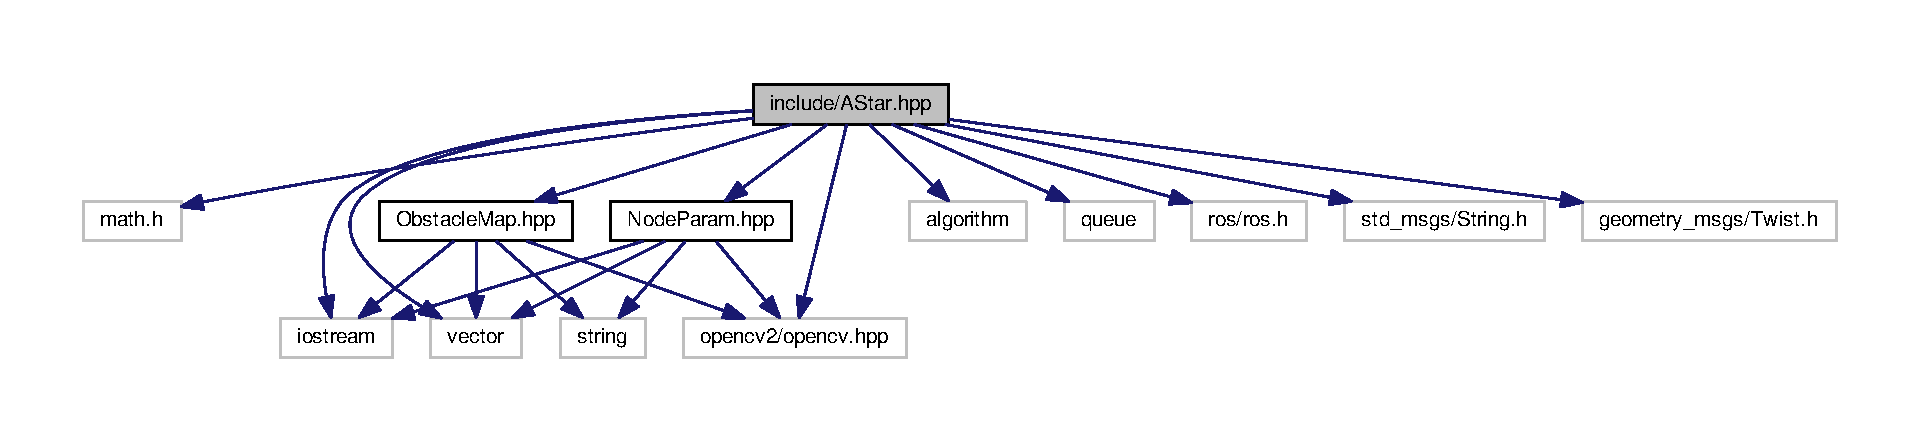
\includegraphics[width=350pt]{_a_star_8hpp__incl}
\end{center}
\end{figure}
This graph shows which files directly or indirectly include this file\+:
\nopagebreak
\begin{figure}[H]
\begin{center}
\leavevmode
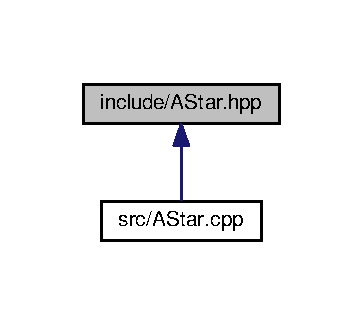
\includegraphics[width=174pt]{_a_star_8hpp__dep__incl}
\end{center}
\end{figure}
\subsection*{Classes}
\begin{DoxyCompactItemize}
\item 
class \hyperlink{class_a_star}{A\+Star}
\begin{DoxyCompactList}\small\item\em \hyperlink{class_a_star}{A\+Star} class Class for the implementation of A$\ast$ algorithm. \end{DoxyCompactList}\end{DoxyCompactItemize}


\subsection{Detailed Description}
Header file for \hyperlink{_a_star_8cpp}{A\+Star.\+cpp} Defines the member variables and functions in \hyperlink{class_a_star}{A\+Star} class. 

The 3-\/\+Clause B\+SD License

Copyright (c) 2019, Ishan Patel, Nakul Patel, Sri Manika Makam

Redistribution and use in source and binary forms, with or without modification, are permitted provided that the following conditions are met\+:


\begin{DoxyEnumerate}
\item Redistributions of source code must retain the above copyright notice, this list of conditions and the following disclaimer.
\item Redistributions in binary form must reproduce the above copyright notice, this list of conditions and the following disclaimer in the documentation and/or other materials provided with the distribution.
\item Neither the name of the copyright holder nor the names of its contributors may be used to endorse or promote products derived from this software without specific prior written permission.
\end{DoxyEnumerate}

T\+H\+IS S\+O\+F\+T\+W\+A\+RE IS P\+R\+O\+V\+I\+D\+ED BY T\+HE C\+O\+P\+Y\+R\+I\+G\+HT H\+O\+L\+D\+E\+RS A\+ND C\+O\+N\+T\+R\+I\+B\+U\+T\+O\+RS \char`\"{}\+A\+S
\+I\+S\char`\"{} A\+ND A\+NY E\+X\+P\+R\+E\+SS OR I\+M\+P\+L\+I\+ED W\+A\+R\+R\+A\+N\+T\+I\+ES, I\+N\+C\+L\+U\+D\+I\+NG, B\+UT N\+OT L\+I\+M\+I\+T\+ED TO, T\+HE I\+M\+P\+L\+I\+ED W\+A\+R\+R\+A\+N\+T\+I\+ES OF M\+E\+R\+C\+H\+A\+N\+T\+A\+B\+I\+L\+I\+TY A\+ND F\+I\+T\+N\+E\+SS F\+OR A P\+A\+R\+T\+I\+C\+U\+L\+AR P\+U\+R\+P\+O\+SE A\+RE D\+I\+S\+C\+L\+A\+I\+M\+ED. IN NO E\+V\+E\+NT S\+H\+A\+LL T\+HE C\+O\+P\+Y\+R\+I\+G\+HT H\+O\+L\+D\+ER OR C\+O\+N\+T\+R\+I\+B\+U\+T\+O\+RS BE L\+I\+A\+B\+LE F\+OR A\+NY D\+I\+R\+E\+CT, I\+N\+D\+I\+R\+E\+CT, I\+N\+C\+I\+D\+E\+N\+T\+AL, S\+P\+E\+C\+I\+AL, E\+X\+E\+M\+P\+L\+A\+RY, OR C\+O\+N\+S\+E\+Q\+U\+E\+N\+T\+I\+AL D\+A\+M\+A\+G\+ES (I\+N\+C\+L\+U\+D\+I\+NG, B\+UT N\+OT L\+I\+M\+I\+T\+ED TO, P\+R\+O\+C\+U\+R\+E\+M\+E\+NT OF S\+U\+B\+S\+T\+I\+T\+U\+TE G\+O\+O\+DS OR S\+E\+R\+V\+I\+C\+ES; L\+O\+SS OF U\+SE, D\+A\+TA, OR P\+R\+O\+F\+I\+TS; OR B\+U\+S\+I\+N\+E\+SS I\+N\+T\+E\+R\+R\+U\+P\+T\+I\+ON) H\+O\+W\+E\+V\+ER C\+A\+U\+S\+ED A\+ND ON A\+NY T\+H\+E\+O\+RY OF L\+I\+A\+B\+I\+L\+I\+TY, W\+H\+E\+T\+H\+ER IN C\+O\+N\+T\+R\+A\+CT, S\+T\+R\+I\+CT L\+I\+A\+B\+I\+L\+I\+TY, OR T\+O\+RT (I\+N\+C\+L\+U\+D\+I\+NG N\+E\+G\+L\+I\+G\+E\+N\+CE OR O\+T\+H\+E\+R\+W\+I\+SE) A\+R\+I\+S\+I\+NG IN A\+NY W\+AY O\+UT OF T\+HE U\+SE OF T\+H\+IS S\+O\+F\+T\+W\+A\+RE, E\+V\+EN IF A\+D\+V\+I\+S\+ED OF

\begin{DoxyAuthor}{Author}
Ishan Patel 
\end{DoxyAuthor}
\begin{DoxyCopyright}{Copyright}
3-\/\+Clause B\+SD License 
\end{DoxyCopyright}

\hypertarget{_node_param_8hpp}{}\section{include/\+Node\+Param.hpp File Reference}
\label{_node_param_8hpp}\index{include/\+Node\+Param.\+hpp@{include/\+Node\+Param.\+hpp}}


Header file for Node\+Param.\+cpp Defines the member variables and functions in \hyperlink{class_node_param}{Node\+Param} class.  


{\ttfamily \#include $<$iostream$>$}\\*
{\ttfamily \#include $<$string$>$}\\*
{\ttfamily \#include $<$vector$>$}\\*
{\ttfamily \#include $<$opencv2/opencv.\+hpp$>$}\\*
Include dependency graph for Node\+Param.\+hpp\+:
\nopagebreak
\begin{figure}[H]
\begin{center}
\leavevmode
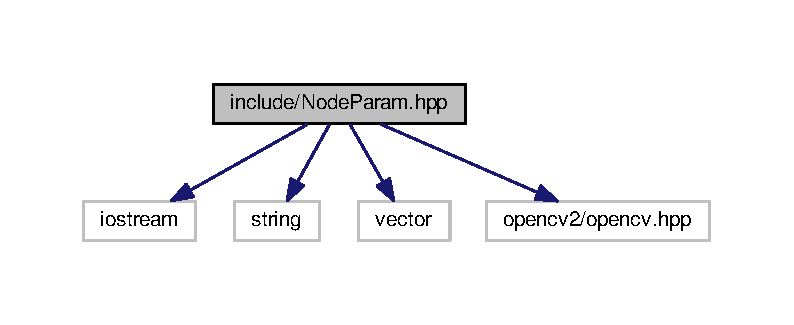
\includegraphics[width=350pt]{_node_param_8hpp__incl}
\end{center}
\end{figure}
This graph shows which files directly or indirectly include this file\+:
\nopagebreak
\begin{figure}[H]
\begin{center}
\leavevmode
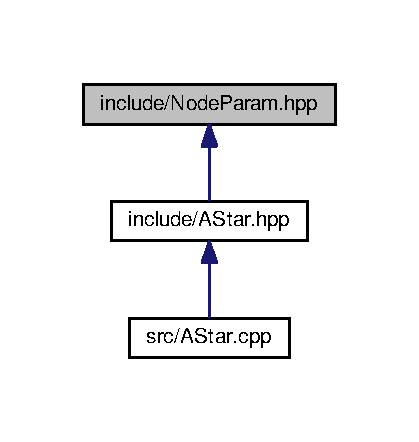
\includegraphics[width=201pt]{_node_param_8hpp__dep__incl}
\end{center}
\end{figure}
\subsection*{Classes}
\begin{DoxyCompactItemize}
\item 
class \hyperlink{class_node_param}{Node\+Param}
\begin{DoxyCompactList}\small\item\em \hyperlink{class_node_param}{Node\+Param} class Class for the implementation of costs, velocities, angles and coordinates for nodes in A$\ast$ algorithm. \end{DoxyCompactList}\end{DoxyCompactItemize}


\subsection{Detailed Description}
Header file for Node\+Param.\+cpp Defines the member variables and functions in \hyperlink{class_node_param}{Node\+Param} class. 

The 3-\/\+Clause B\+SD License

Copyright (c) 2019, Ishan Patel, Nakul Patel, Sri Manika Makam

Redistribution and use in source and binary forms, with or without modification, are permitted provided that the following conditions are met\+:


\begin{DoxyEnumerate}
\item Redistributions of source code must retain the above copyright notice, this list of conditions and the following disclaimer.
\item Redistributions in binary form must reproduce the above copyright notice, this list of conditions and the following disclaimer in the documentation and/or other materials provided with the distribution.
\item Neither the name of the copyright holder nor the names of its contributors may be used to endorse or promote products derived from this software without specific prior written permission.
\end{DoxyEnumerate}

T\+H\+IS S\+O\+F\+T\+W\+A\+RE IS P\+R\+O\+V\+I\+D\+ED BY T\+HE C\+O\+P\+Y\+R\+I\+G\+HT H\+O\+L\+D\+E\+RS A\+ND C\+O\+N\+T\+R\+I\+B\+U\+T\+O\+RS \char`\"{}\+A\+S
\+I\+S\char`\"{} A\+ND A\+NY E\+X\+P\+R\+E\+SS OR I\+M\+P\+L\+I\+ED W\+A\+R\+R\+A\+N\+T\+I\+ES, I\+N\+C\+L\+U\+D\+I\+NG, B\+UT N\+OT L\+I\+M\+I\+T\+ED TO, T\+HE I\+M\+P\+L\+I\+ED W\+A\+R\+R\+A\+N\+T\+I\+ES OF M\+E\+R\+C\+H\+A\+N\+T\+A\+B\+I\+L\+I\+TY A\+ND F\+I\+T\+N\+E\+SS F\+OR A P\+A\+R\+T\+I\+C\+U\+L\+AR P\+U\+R\+P\+O\+SE A\+RE D\+I\+S\+C\+L\+A\+I\+M\+ED. IN NO E\+V\+E\+NT S\+H\+A\+LL T\+HE C\+O\+P\+Y\+R\+I\+G\+HT H\+O\+L\+D\+ER OR C\+O\+N\+T\+R\+I\+B\+U\+T\+O\+RS BE L\+I\+A\+B\+LE F\+OR A\+NY D\+I\+R\+E\+CT, I\+N\+D\+I\+R\+E\+CT, I\+N\+C\+I\+D\+E\+N\+T\+AL, S\+P\+E\+C\+I\+AL, E\+X\+E\+M\+P\+L\+A\+RY, OR C\+O\+N\+S\+E\+Q\+U\+E\+N\+T\+I\+AL D\+A\+M\+A\+G\+ES (I\+N\+C\+L\+U\+D\+I\+NG, B\+UT N\+OT L\+I\+M\+I\+T\+ED TO, P\+R\+O\+C\+U\+R\+E\+M\+E\+NT OF S\+U\+B\+S\+T\+I\+T\+U\+TE G\+O\+O\+DS OR S\+E\+R\+V\+I\+C\+ES; L\+O\+SS OF U\+SE, D\+A\+TA, OR P\+R\+O\+F\+I\+TS; OR B\+U\+S\+I\+N\+E\+SS I\+N\+T\+E\+R\+R\+U\+P\+T\+I\+ON) H\+O\+W\+E\+V\+ER C\+A\+U\+S\+ED A\+ND ON A\+NY T\+H\+E\+O\+RY OF L\+I\+A\+B\+I\+L\+I\+TY, W\+H\+E\+T\+H\+ER IN C\+O\+N\+T\+R\+A\+CT, S\+T\+R\+I\+CT L\+I\+A\+B\+I\+L\+I\+TY, OR T\+O\+RT (I\+N\+C\+L\+U\+D\+I\+NG N\+E\+G\+L\+I\+G\+E\+N\+CE OR O\+T\+H\+E\+R\+W\+I\+SE) A\+R\+I\+S\+I\+NG IN A\+NY W\+AY O\+UT OF T\+HE U\+SE OF T\+H\+IS S\+O\+F\+T\+W\+A\+RE, E\+V\+EN IF A\+D\+V\+I\+S\+ED OF

\begin{DoxyAuthor}{Author}
Sri Manika Makam 
\end{DoxyAuthor}
\begin{DoxyCopyright}{Copyright}
3-\/\+Clause B\+SD License 
\end{DoxyCopyright}

\hypertarget{_obstacle_map_8hpp}{}\section{include/\+Obstacle\+Map.hpp File Reference}
\label{_obstacle_map_8hpp}\index{include/\+Obstacle\+Map.\+hpp@{include/\+Obstacle\+Map.\+hpp}}


Header file for \hyperlink{_obstacle_map_8cpp}{Obstacle\+Map.\+cpp} Defines the member variables and functions in \hyperlink{class_obstacle_map}{Obstacle\+Map} class.  


{\ttfamily \#include $<$iostream$>$}\\*
{\ttfamily \#include $<$string$>$}\\*
{\ttfamily \#include $<$vector$>$}\\*
{\ttfamily \#include $<$opencv2/opencv.\+hpp$>$}\\*
Include dependency graph for Obstacle\+Map.\+hpp\+:
\nopagebreak
\begin{figure}[H]
\begin{center}
\leavevmode
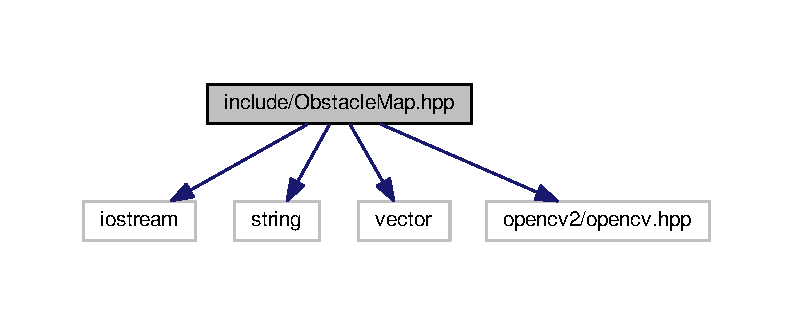
\includegraphics[width=350pt]{_obstacle_map_8hpp__incl}
\end{center}
\end{figure}
This graph shows which files directly or indirectly include this file\+:
\nopagebreak
\begin{figure}[H]
\begin{center}
\leavevmode
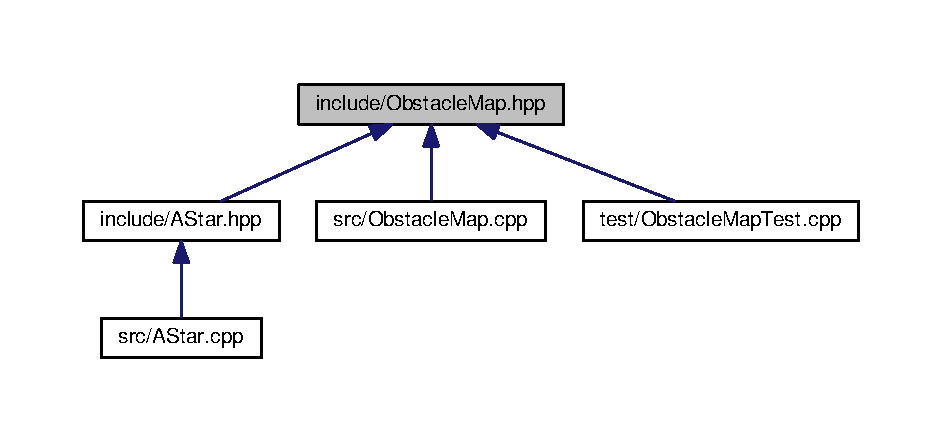
\includegraphics[width=350pt]{_obstacle_map_8hpp__dep__incl}
\end{center}
\end{figure}
\subsection*{Classes}
\begin{DoxyCompactItemize}
\item 
class \hyperlink{class_obstacle_map}{Obstacle\+Map}
\begin{DoxyCompactList}\small\item\em \hyperlink{class_obstacle_map}{Obstacle\+Map} class Class for the implementation of obstacle map. \end{DoxyCompactList}\end{DoxyCompactItemize}


\subsection{Detailed Description}
Header file for \hyperlink{_obstacle_map_8cpp}{Obstacle\+Map.\+cpp} Defines the member variables and functions in \hyperlink{class_obstacle_map}{Obstacle\+Map} class. 

The 3-\/\+Clause B\+SD License

Copyright (c) 2019, Ishan Patel, Nakul Patel, Sri Manika Makam

Redistribution and use in source and binary forms, with or without modification, are permitted provided that the following conditions are met\+:


\begin{DoxyEnumerate}
\item Redistributions of source code must retain the above copyright notice, this list of conditions and the following disclaimer.
\item Redistributions in binary form must reproduce the above copyright notice, this list of conditions and the following disclaimer in the documentation and/or other materials provided with the distribution.
\item Neither the name of the copyright holder nor the names of its contributors may be used to endorse or promote products derived from this software without specific prior written permission.
\end{DoxyEnumerate}

T\+H\+IS S\+O\+F\+T\+W\+A\+RE IS P\+R\+O\+V\+I\+D\+ED BY T\+HE C\+O\+P\+Y\+R\+I\+G\+HT H\+O\+L\+D\+E\+RS A\+ND C\+O\+N\+T\+R\+I\+B\+U\+T\+O\+RS \char`\"{}\+A\+S
\+I\+S\char`\"{} A\+ND A\+NY E\+X\+P\+R\+E\+SS OR I\+M\+P\+L\+I\+ED W\+A\+R\+R\+A\+N\+T\+I\+ES, I\+N\+C\+L\+U\+D\+I\+NG, B\+UT N\+OT L\+I\+M\+I\+T\+ED TO, T\+HE I\+M\+P\+L\+I\+ED W\+A\+R\+R\+A\+N\+T\+I\+ES OF M\+E\+R\+C\+H\+A\+N\+T\+A\+B\+I\+L\+I\+TY A\+ND F\+I\+T\+N\+E\+SS F\+OR A P\+A\+R\+T\+I\+C\+U\+L\+AR P\+U\+R\+P\+O\+SE A\+RE D\+I\+S\+C\+L\+A\+I\+M\+ED. IN NO E\+V\+E\+NT S\+H\+A\+LL T\+HE C\+O\+P\+Y\+R\+I\+G\+HT H\+O\+L\+D\+ER OR C\+O\+N\+T\+R\+I\+B\+U\+T\+O\+RS BE L\+I\+A\+B\+LE F\+OR A\+NY D\+I\+R\+E\+CT, I\+N\+D\+I\+R\+E\+CT, I\+N\+C\+I\+D\+E\+N\+T\+AL, S\+P\+E\+C\+I\+AL, E\+X\+E\+M\+P\+L\+A\+RY, OR C\+O\+N\+S\+E\+Q\+U\+E\+N\+T\+I\+AL D\+A\+M\+A\+G\+ES (I\+N\+C\+L\+U\+D\+I\+NG, B\+UT N\+OT L\+I\+M\+I\+T\+ED TO, P\+R\+O\+C\+U\+R\+E\+M\+E\+NT OF S\+U\+B\+S\+T\+I\+T\+U\+TE G\+O\+O\+DS OR S\+E\+R\+V\+I\+C\+ES; L\+O\+SS OF U\+SE, D\+A\+TA, OR P\+R\+O\+F\+I\+TS; OR B\+U\+S\+I\+N\+E\+SS I\+N\+T\+E\+R\+R\+U\+P\+T\+I\+ON) H\+O\+W\+E\+V\+ER C\+A\+U\+S\+ED A\+ND ON A\+NY T\+H\+E\+O\+RY OF L\+I\+A\+B\+I\+L\+I\+TY, W\+H\+E\+T\+H\+ER IN C\+O\+N\+T\+R\+A\+CT, S\+T\+R\+I\+CT L\+I\+A\+B\+I\+L\+I\+TY, OR T\+O\+RT (I\+N\+C\+L\+U\+D\+I\+NG N\+E\+G\+L\+I\+G\+E\+N\+CE OR O\+T\+H\+E\+R\+W\+I\+SE) A\+R\+I\+S\+I\+NG IN A\+NY W\+AY O\+UT OF T\+HE U\+SE OF T\+H\+IS S\+O\+F\+T\+W\+A\+RE, E\+V\+EN IF A\+D\+V\+I\+S\+ED OF

\begin{DoxyAuthor}{Author}
Nakul Patel 
\end{DoxyAuthor}
\begin{DoxyCopyright}{Copyright}
3-\/\+Clause B\+SD License 
\end{DoxyCopyright}

\hypertarget{_a_star_8cpp}{}\section{src/\+A\+Star.cpp File Reference}
\label{_a_star_8cpp}\index{src/\+A\+Star.\+cpp@{src/\+A\+Star.\+cpp}}


Implementation of \hyperlink{class_a_star}{A\+Star} class.  


{\ttfamily \#include \char`\"{}A\+Star.\+hpp\char`\"{}}\\*
{\ttfamily \#include $<$math.\+h$>$}\\*
{\ttfamily \#include $<$iostream$>$}\\*
{\ttfamily \#include $<$vector$>$}\\*
{\ttfamily \#include $<$algorithm$>$}\\*
{\ttfamily \#include $<$queue$>$}\\*
{\ttfamily \#include $<$opencv2/opencv.\+hpp$>$}\\*
{\ttfamily \#include \char`\"{}ros/ros.\+h\char`\"{}}\\*
{\ttfamily \#include \char`\"{}std\+\_\+msgs/\+String.\+h\char`\"{}}\\*
{\ttfamily \#include \char`\"{}geometry\+\_\+msgs/\+Twist.\+h\char`\"{}}\\*
Include dependency graph for A\+Star.\+cpp\+:
\nopagebreak
\begin{figure}[H]
\begin{center}
\leavevmode
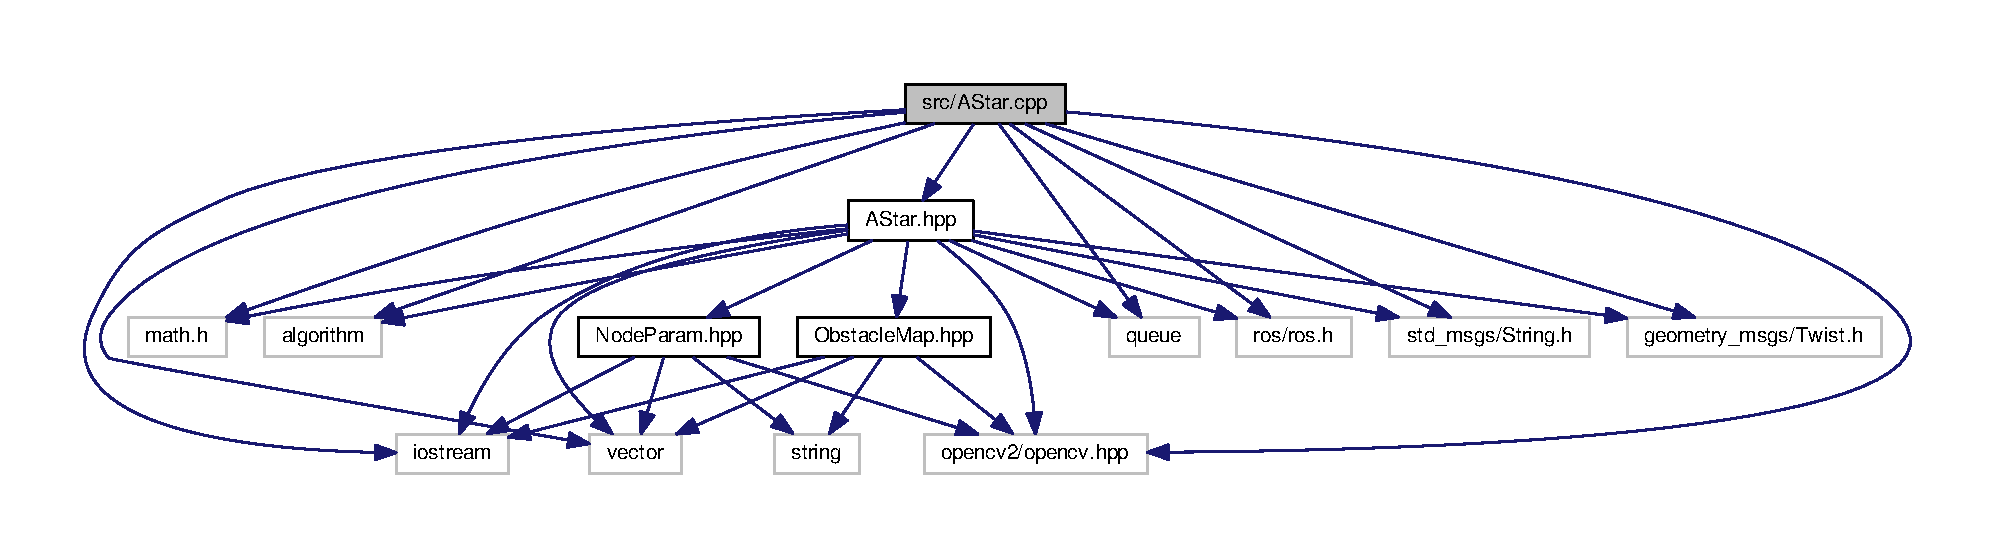
\includegraphics[width=350pt]{_a_star_8cpp__incl}
\end{center}
\end{figure}
\subsection*{Typedefs}
\begin{DoxyCompactItemize}
\item 
typedef std\+::vector$<$ std\+::vector$<$ std\+::vector$<$ double $>$ $>$ $>$ \hyperlink{_a_star_8cpp_a4322c2160c88baf9e32aa9a685dd4769}{nest\+Vector}
\end{DoxyCompactItemize}


\subsection{Detailed Description}
Implementation of \hyperlink{class_a_star}{A\+Star} class. 

The 3-\/\+Clause B\+SD License

Copyright (c) 2019, Ishan Patel, Nakul Patel, Sri Manika Makam

Redistribution and use in source and binary forms, with or without modification, are permitted provided that the following conditions are met\+:


\begin{DoxyEnumerate}
\item Redistributions of source code must retain the above copyright notice, this list of conditions and the following disclaimer.
\item Redistributions in binary form must reproduce the above copyright notice, this list of conditions and the following disclaimer in the documentation and/or other materials provided with the distribution.
\item Neither the name of the copyright holder nor the names of its contributors may be used to endorse or promote products derived from this software without specific prior written permission.
\end{DoxyEnumerate}

T\+H\+IS S\+O\+F\+T\+W\+A\+RE IS P\+R\+O\+V\+I\+D\+ED BY T\+HE C\+O\+P\+Y\+R\+I\+G\+HT H\+O\+L\+D\+E\+RS A\+ND C\+O\+N\+T\+R\+I\+B\+U\+T\+O\+RS \char`\"{}\+A\+S
\+I\+S\char`\"{} A\+ND A\+NY E\+X\+P\+R\+E\+SS OR I\+M\+P\+L\+I\+ED W\+A\+R\+R\+A\+N\+T\+I\+ES, I\+N\+C\+L\+U\+D\+I\+NG, B\+UT N\+OT L\+I\+M\+I\+T\+ED TO, T\+HE I\+M\+P\+L\+I\+ED W\+A\+R\+R\+A\+N\+T\+I\+ES OF M\+E\+R\+C\+H\+A\+N\+T\+A\+B\+I\+L\+I\+TY A\+ND F\+I\+T\+N\+E\+SS F\+OR A P\+A\+R\+T\+I\+C\+U\+L\+AR P\+U\+R\+P\+O\+SE A\+RE D\+I\+S\+C\+L\+A\+I\+M\+ED. IN NO E\+V\+E\+NT S\+H\+A\+LL T\+HE C\+O\+P\+Y\+R\+I\+G\+HT H\+O\+L\+D\+ER OR C\+O\+N\+T\+R\+I\+B\+U\+T\+O\+RS BE L\+I\+A\+B\+LE F\+OR A\+NY D\+I\+R\+E\+CT, I\+N\+D\+I\+R\+E\+CT, I\+N\+C\+I\+D\+E\+N\+T\+AL, S\+P\+E\+C\+I\+AL, E\+X\+E\+M\+P\+L\+A\+RY, OR C\+O\+N\+S\+E\+Q\+U\+E\+N\+T\+I\+AL D\+A\+M\+A\+G\+ES (I\+N\+C\+L\+U\+D\+I\+NG, B\+UT N\+OT L\+I\+M\+I\+T\+ED TO, P\+R\+O\+C\+U\+R\+E\+M\+E\+NT OF S\+U\+B\+S\+T\+I\+T\+U\+TE G\+O\+O\+DS OR S\+E\+R\+V\+I\+C\+ES; L\+O\+SS OF U\+SE, D\+A\+TA, OR P\+R\+O\+F\+I\+TS; OR B\+U\+S\+I\+N\+E\+SS I\+N\+T\+E\+R\+R\+U\+P\+T\+I\+ON) H\+O\+W\+E\+V\+ER C\+A\+U\+S\+ED A\+ND ON A\+NY T\+H\+E\+O\+RY OF L\+I\+A\+B\+I\+L\+I\+TY, W\+H\+E\+T\+H\+ER IN C\+O\+N\+T\+R\+A\+CT, S\+T\+R\+I\+CT L\+I\+A\+B\+I\+L\+I\+TY, OR T\+O\+RT (I\+N\+C\+L\+U\+D\+I\+NG N\+E\+G\+L\+I\+G\+E\+N\+CE OR O\+T\+H\+E\+R\+W\+I\+SE) A\+R\+I\+S\+I\+NG IN A\+NY W\+AY O\+UT OF T\+HE U\+SE OF T\+H\+IS S\+O\+F\+T\+W\+A\+RE, E\+V\+EN IF A\+D\+V\+I\+S\+ED OF

\begin{DoxyAuthor}{Author}
Ishan Patel 
\end{DoxyAuthor}
\begin{DoxyCopyright}{Copyright}
3-\/\+Clause B\+SD License 
\end{DoxyCopyright}


\subsection{Typedef Documentation}
\index{A\+Star.\+cpp@{A\+Star.\+cpp}!nest\+Vector@{nest\+Vector}}
\index{nest\+Vector@{nest\+Vector}!A\+Star.\+cpp@{A\+Star.\+cpp}}
\subsubsection[{\texorpdfstring{nest\+Vector}{nestVector}}]{\setlength{\rightskip}{0pt plus 5cm}typedef std\+::vector$<$std\+::vector$<$std\+::vector$<$double$>$ $>$ $>$ {\bf nest\+Vector}}\hypertarget{_a_star_8cpp_a4322c2160c88baf9e32aa9a685dd4769}{}\label{_a_star_8cpp_a4322c2160c88baf9e32aa9a685dd4769}
declaring typedef for std\+::vector$<$std\+::vector$<$std\+::vector$<$double$>$$>$$>$ 
\hypertarget{_obstacle_map_8cpp}{}\section{src/\+Obstacle\+Map.cpp File Reference}
\label{_obstacle_map_8cpp}\index{src/\+Obstacle\+Map.\+cpp@{src/\+Obstacle\+Map.\+cpp}}


Header file for \hyperlink{_obstacle_map_8cpp}{Obstacle\+Map.\+cpp}.  


{\ttfamily \#include \char`\"{}Obstacle\+Map.\+hpp\char`\"{}}\\*
{\ttfamily \#include $<$iostream$>$}\\*
{\ttfamily \#include $<$string$>$}\\*
{\ttfamily \#include $<$vector$>$}\\*
{\ttfamily \#include $<$opencv2/opencv.\+hpp$>$}\\*
Include dependency graph for Obstacle\+Map.\+cpp\+:
\nopagebreak
\begin{figure}[H]
\begin{center}
\leavevmode
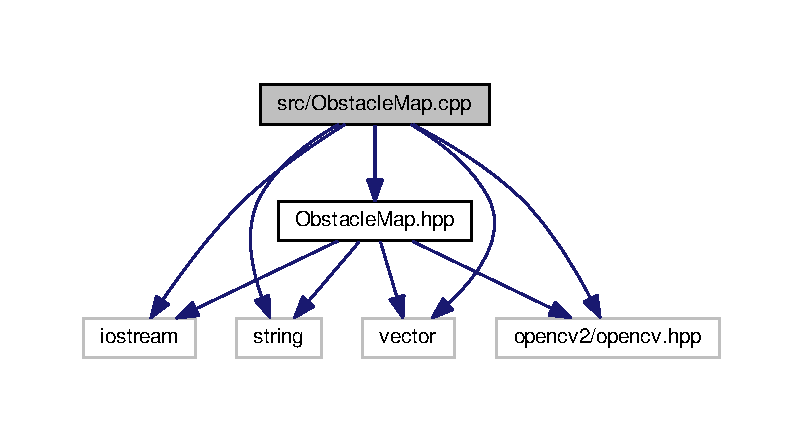
\includegraphics[width=350pt]{_obstacle_map_8cpp__incl}
\end{center}
\end{figure}


\subsection{Detailed Description}
Header file for \hyperlink{_obstacle_map_8cpp}{Obstacle\+Map.\+cpp}. 

The 3-\/\+Clause B\+SD License

Copyright (c) 2019, Ishan Patel, Nakul Patel, Sri Manika Makam

Redistribution and use in source and binary forms, with or without modification, are permitted provided that the following conditions are met\+:


\begin{DoxyEnumerate}
\item Redistributions of source code must retain the above copyright notice, this list of conditions and the following disclaimer.
\item Redistributions in binary form must reproduce the above copyright notice, this list of conditions and the following disclaimer in the documentation and/or other materials provided with the distribution.
\item Neither the name of the copyright holder nor the names of its contributors may be used to endorse or promote products derived from this software without specific prior written permission.
\end{DoxyEnumerate}

T\+H\+IS S\+O\+F\+T\+W\+A\+RE IS P\+R\+O\+V\+I\+D\+ED BY T\+HE C\+O\+P\+Y\+R\+I\+G\+HT H\+O\+L\+D\+E\+RS A\+ND C\+O\+N\+T\+R\+I\+B\+U\+T\+O\+RS \char`\"{}\+A\+S
\+I\+S\char`\"{} A\+ND A\+NY E\+X\+P\+R\+E\+SS OR I\+M\+P\+L\+I\+ED W\+A\+R\+R\+A\+N\+T\+I\+ES, I\+N\+C\+L\+U\+D\+I\+NG, B\+UT N\+OT L\+I\+M\+I\+T\+ED TO, T\+HE I\+M\+P\+L\+I\+ED W\+A\+R\+R\+A\+N\+T\+I\+ES OF M\+E\+R\+C\+H\+A\+N\+T\+A\+B\+I\+L\+I\+TY A\+ND F\+I\+T\+N\+E\+SS F\+OR A P\+A\+R\+T\+I\+C\+U\+L\+AR P\+U\+R\+P\+O\+SE A\+RE D\+I\+S\+C\+L\+A\+I\+M\+ED. IN NO E\+V\+E\+NT S\+H\+A\+LL T\+HE C\+O\+P\+Y\+R\+I\+G\+HT H\+O\+L\+D\+ER OR C\+O\+N\+T\+R\+I\+B\+U\+T\+O\+RS BE L\+I\+A\+B\+LE F\+OR A\+NY D\+I\+R\+E\+CT, I\+N\+D\+I\+R\+E\+CT, I\+N\+C\+I\+D\+E\+N\+T\+AL, S\+P\+E\+C\+I\+AL, E\+X\+E\+M\+P\+L\+A\+RY, OR C\+O\+N\+S\+E\+Q\+U\+E\+N\+T\+I\+AL D\+A\+M\+A\+G\+ES (I\+N\+C\+L\+U\+D\+I\+NG, B\+UT N\+OT L\+I\+M\+I\+T\+ED TO, P\+R\+O\+C\+U\+R\+E\+M\+E\+NT OF S\+U\+B\+S\+T\+I\+T\+U\+TE G\+O\+O\+DS OR S\+E\+R\+V\+I\+C\+ES; L\+O\+SS OF U\+SE, D\+A\+TA, OR P\+R\+O\+F\+I\+TS; OR B\+U\+S\+I\+N\+E\+SS I\+N\+T\+E\+R\+R\+U\+P\+T\+I\+ON) H\+O\+W\+E\+V\+ER C\+A\+U\+S\+ED A\+ND ON A\+NY T\+H\+E\+O\+RY OF L\+I\+A\+B\+I\+L\+I\+TY, W\+H\+E\+T\+H\+ER IN C\+O\+N\+T\+R\+A\+CT, S\+T\+R\+I\+CT L\+I\+A\+B\+I\+L\+I\+TY, OR T\+O\+RT (I\+N\+C\+L\+U\+D\+I\+NG N\+E\+G\+L\+I\+G\+E\+N\+CE OR O\+T\+H\+E\+R\+W\+I\+SE) A\+R\+I\+S\+I\+NG IN A\+NY W\+AY O\+UT OF T\+HE U\+SE OF T\+H\+IS S\+O\+F\+T\+W\+A\+RE, E\+V\+EN IF A\+D\+V\+I\+S\+ED OF

\begin{DoxyAuthor}{Author}
Nakul Patel 
\end{DoxyAuthor}
\begin{DoxyCopyright}{Copyright}
3-\/\+Clause B\+SD License 
\end{DoxyCopyright}
\hypertarget{_obstacle_map_8cpp_DESCRIPTION}{}\subsection{D\+E\+S\+C\+R\+I\+P\+T\+I\+ON}\label{_obstacle_map_8cpp_DESCRIPTION}
Defines the member variables and functions in \hyperlink{class_obstacle_map}{Obstacle\+Map} class. 
\hypertarget{_obstacle_map_test_8cpp}{}\section{test/\+Obstacle\+Map\+Test.cpp File Reference}
\label{_obstacle_map_test_8cpp}\index{test/\+Obstacle\+Map\+Test.\+cpp@{test/\+Obstacle\+Map\+Test.\+cpp}}


unit tests for \hyperlink{class_a_star}{A\+Star} class  


{\ttfamily \#include $<$ros/ros.\+h$>$}\\*
{\ttfamily \#include $<$gtest/gtest.\+h$>$}\\*
{\ttfamily \#include $<$iostream$>$}\\*
{\ttfamily \#include $<$opencv2/opencv.\+hpp$>$}\\*
{\ttfamily \#include \char`\"{}Obstacle\+Map.\+hpp\char`\"{}}\\*
Include dependency graph for Obstacle\+Map\+Test.\+cpp\+:
\nopagebreak
\begin{figure}[H]
\begin{center}
\leavevmode
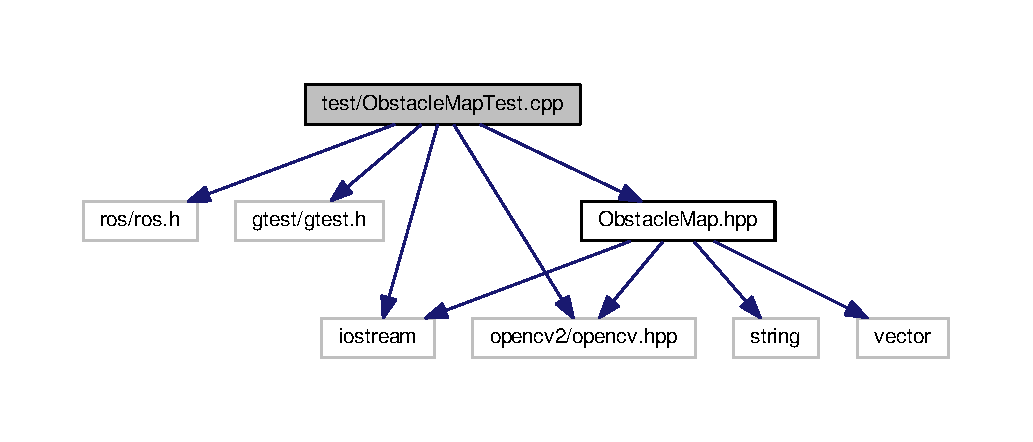
\includegraphics[width=350pt]{_obstacle_map_test_8cpp__incl}
\end{center}
\end{figure}
\subsection*{Functions}
\begin{DoxyCompactItemize}
\item 
\hyperlink{_obstacle_map_test_8cpp_aca2a83cec118a500836e24c93d5ddfab}{T\+E\+ST} (Obstacle\+Map\+Test, Get\+Radius\+Test)
\begin{DoxyCompactList}\small\item\em Test for get\+Radius() function. \end{DoxyCompactList}\item 
\hyperlink{_obstacle_map_test_8cpp_aedbc2811c604dc8050213a700d8d26c2}{T\+E\+ST} (Obstacle\+Map\+Test, Create\+Rectangles\+Test)
\begin{DoxyCompactList}\small\item\em Test for create\+Rectangles() function. \end{DoxyCompactList}\item 
\hyperlink{_obstacle_map_test_8cpp_a3998eed8f531690f0e6c4145e344c78e}{T\+E\+ST} (Obstacle\+Map\+Test, Create\+Tables\+Test)
\begin{DoxyCompactList}\small\item\em Test for create\+Tables() function. \end{DoxyCompactList}\item 
\hyperlink{_obstacle_map_test_8cpp_a609dffea559a9d81cd55453136fd7a30}{T\+E\+ST} (Obstacle\+Map\+Test, Create\+Circles\+Test)
\begin{DoxyCompactList}\small\item\em Test for create\+Circles() function. \end{DoxyCompactList}\item 
\hyperlink{_obstacle_map_test_8cpp_a93e8a31f9279507eddc7d1bc1459ae87}{T\+E\+ST} (Obstacle\+Map\+Test, Draw\+Boundary\+Test)
\begin{DoxyCompactList}\small\item\em Test for draw\+Boundary() function. \end{DoxyCompactList}\item 
\hyperlink{_obstacle_map_test_8cpp_aef0f55b85777bc9a1098059cf658ae5f}{T\+E\+ST} (Obstacle\+Map\+Test, Create\+Map\+Test)
\begin{DoxyCompactList}\small\item\em Test for create\+Map() function. \end{DoxyCompactList}\end{DoxyCompactItemize}


\subsection{Detailed Description}
unit tests for \hyperlink{class_a_star}{A\+Star} class 

unit tests for \hyperlink{class_obstacle_map}{Obstacle\+Map} class

The 3-\/\+Clause B\+SD License

Copyright (c) 2019, Ishan Patel, Nakul Patel, Sri Manika Makam

Redistribution and use in source and binary forms, with or without modification, are permitted provided that the following conditions are met\+:


\begin{DoxyEnumerate}
\item Redistributions of source code must retain the above copyright notice, this list of conditions and the following disclaimer.
\item Redistributions in binary form must reproduce the above copyright notice, this list of conditions and the following disclaimer in the documentation and/or other materials provided with the distribution.
\item Neither the name of the copyright holder nor the names of its contributors may be used to endorse or promote products derived from this software without specific prior written permission.
\end{DoxyEnumerate}

T\+H\+IS S\+O\+F\+T\+W\+A\+RE IS P\+R\+O\+V\+I\+D\+ED BY T\+HE C\+O\+P\+Y\+R\+I\+G\+HT H\+O\+L\+D\+E\+RS A\+ND C\+O\+N\+T\+R\+I\+B\+U\+T\+O\+RS \char`\"{}\+A\+S
\+I\+S\char`\"{} A\+ND A\+NY E\+X\+P\+R\+E\+SS OR I\+M\+P\+L\+I\+ED W\+A\+R\+R\+A\+N\+T\+I\+ES, I\+N\+C\+L\+U\+D\+I\+NG, B\+UT N\+OT L\+I\+M\+I\+T\+ED TO, T\+HE I\+M\+P\+L\+I\+ED W\+A\+R\+R\+A\+N\+T\+I\+ES OF M\+E\+R\+C\+H\+A\+N\+T\+A\+B\+I\+L\+I\+TY A\+ND F\+I\+T\+N\+E\+SS F\+OR A P\+A\+R\+T\+I\+C\+U\+L\+AR P\+U\+R\+P\+O\+SE A\+RE D\+I\+S\+C\+L\+A\+I\+M\+ED. IN NO E\+V\+E\+NT S\+H\+A\+LL T\+HE C\+O\+P\+Y\+R\+I\+G\+HT H\+O\+L\+D\+ER OR C\+O\+N\+T\+R\+I\+B\+U\+T\+O\+RS BE L\+I\+A\+B\+LE F\+OR A\+NY D\+I\+R\+E\+CT, I\+N\+D\+I\+R\+E\+CT, I\+N\+C\+I\+D\+E\+N\+T\+AL, S\+P\+E\+C\+I\+AL, E\+X\+E\+M\+P\+L\+A\+RY, OR C\+O\+N\+S\+E\+Q\+U\+E\+N\+T\+I\+AL D\+A\+M\+A\+G\+ES (I\+N\+C\+L\+U\+D\+I\+NG, B\+UT N\+OT L\+I\+M\+I\+T\+ED TO, P\+R\+O\+C\+U\+R\+E\+M\+E\+NT OF S\+U\+B\+S\+T\+I\+T\+U\+TE G\+O\+O\+DS OR S\+E\+R\+V\+I\+C\+ES; L\+O\+SS OF U\+SE, D\+A\+TA, OR P\+R\+O\+F\+I\+TS; OR B\+U\+S\+I\+N\+E\+SS I\+N\+T\+E\+R\+R\+U\+P\+T\+I\+ON) H\+O\+W\+E\+V\+ER C\+A\+U\+S\+ED A\+ND ON A\+NY T\+H\+E\+O\+RY OF L\+I\+A\+B\+I\+L\+I\+TY, W\+H\+E\+T\+H\+ER IN C\+O\+N\+T\+R\+A\+CT, S\+T\+R\+I\+CT L\+I\+A\+B\+I\+L\+I\+TY, OR T\+O\+RT (I\+N\+C\+L\+U\+D\+I\+NG N\+E\+G\+L\+I\+G\+E\+N\+CE OR O\+T\+H\+E\+R\+W\+I\+SE) A\+R\+I\+S\+I\+NG IN A\+NY W\+AY O\+UT OF T\+HE U\+SE OF T\+H\+IS S\+O\+F\+T\+W\+A\+RE, E\+V\+EN IF A\+D\+V\+I\+S\+ED OF

\begin{DoxyAuthor}{Author}
Ishan Patel 
\end{DoxyAuthor}
\begin{DoxyCopyright}{Copyright}
3-\/\+Clause B\+SD License This is the .cpp file that uses certain unit tests from gtest framework to test the functions of \hyperlink{class_a_star}{A\+Star} class.
\end{DoxyCopyright}
The 3-\/\+Clause B\+SD License

Copyright (c) 2019, Ishan Patel, Nakul Patel, Sri Manika Makam

Redistribution and use in source and binary forms, with or without modification, are permitted provided that the following conditions are met\+:


\begin{DoxyEnumerate}
\item Redistributions of source code must retain the above copyright notice, this list of conditions and the following disclaimer.
\item Redistributions in binary form must reproduce the above copyright notice, this list of conditions and the following disclaimer in the documentation and/or other materials provided with the distribution.
\item Neither the name of the copyright holder nor the names of its contributors may be used to endorse or promote products derived from this software without specific prior written permission.
\end{DoxyEnumerate}

T\+H\+IS S\+O\+F\+T\+W\+A\+RE IS P\+R\+O\+V\+I\+D\+ED BY T\+HE C\+O\+P\+Y\+R\+I\+G\+HT H\+O\+L\+D\+E\+RS A\+ND C\+O\+N\+T\+R\+I\+B\+U\+T\+O\+RS \char`\"{}\+A\+S
\+I\+S\char`\"{} A\+ND A\+NY E\+X\+P\+R\+E\+SS OR I\+M\+P\+L\+I\+ED W\+A\+R\+R\+A\+N\+T\+I\+ES, I\+N\+C\+L\+U\+D\+I\+NG, B\+UT N\+OT L\+I\+M\+I\+T\+ED TO, T\+HE I\+M\+P\+L\+I\+ED W\+A\+R\+R\+A\+N\+T\+I\+ES OF M\+E\+R\+C\+H\+A\+N\+T\+A\+B\+I\+L\+I\+TY A\+ND F\+I\+T\+N\+E\+SS F\+OR A P\+A\+R\+T\+I\+C\+U\+L\+AR P\+U\+R\+P\+O\+SE A\+RE D\+I\+S\+C\+L\+A\+I\+M\+ED. IN NO E\+V\+E\+NT S\+H\+A\+LL T\+HE C\+O\+P\+Y\+R\+I\+G\+HT H\+O\+L\+D\+ER OR C\+O\+N\+T\+R\+I\+B\+U\+T\+O\+RS BE L\+I\+A\+B\+LE F\+OR A\+NY D\+I\+R\+E\+CT, I\+N\+D\+I\+R\+E\+CT, I\+N\+C\+I\+D\+E\+N\+T\+AL, S\+P\+E\+C\+I\+AL, E\+X\+E\+M\+P\+L\+A\+RY, OR C\+O\+N\+S\+E\+Q\+U\+E\+N\+T\+I\+AL D\+A\+M\+A\+G\+ES (I\+N\+C\+L\+U\+D\+I\+NG, B\+UT N\+OT L\+I\+M\+I\+T\+ED TO, P\+R\+O\+C\+U\+R\+E\+M\+E\+NT OF S\+U\+B\+S\+T\+I\+T\+U\+TE G\+O\+O\+DS OR S\+E\+R\+V\+I\+C\+ES; L\+O\+SS OF U\+SE, D\+A\+TA, OR P\+R\+O\+F\+I\+TS; OR B\+U\+S\+I\+N\+E\+SS I\+N\+T\+E\+R\+R\+U\+P\+T\+I\+ON) H\+O\+W\+E\+V\+ER C\+A\+U\+S\+ED A\+ND ON A\+NY T\+H\+E\+O\+RY OF L\+I\+A\+B\+I\+L\+I\+TY, W\+H\+E\+T\+H\+ER IN C\+O\+N\+T\+R\+A\+CT, S\+T\+R\+I\+CT L\+I\+A\+B\+I\+L\+I\+TY, OR T\+O\+RT (I\+N\+C\+L\+U\+D\+I\+NG N\+E\+G\+L\+I\+G\+E\+N\+CE OR O\+T\+H\+E\+R\+W\+I\+SE) A\+R\+I\+S\+I\+NG IN A\+NY W\+AY O\+UT OF T\+HE U\+SE OF T\+H\+IS S\+O\+F\+T\+W\+A\+RE, E\+V\+EN IF A\+D\+V\+I\+S\+ED OF

\begin{DoxyAuthor}{Author}
Sri Manika Makam 
\end{DoxyAuthor}
\begin{DoxyCopyright}{Copyright}
3-\/\+Clause B\+SD License This is the .cpp file that uses certain unit tests from gtest framework to test the functions of \hyperlink{class_node_param}{Node\+Param} class.
\end{DoxyCopyright}
The 3-\/\+Clause B\+SD License

Copyright (c) 2019, Ishan Patel, Nakul Patel, Sri Manika Makam

Redistribution and use in source and binary forms, with or without modification, are permitted provided that the following conditions are met\+:


\begin{DoxyEnumerate}
\item Redistributions of source code must retain the above copyright notice, this list of conditions and the following disclaimer.
\item Redistributions in binary form must reproduce the above copyright notice, this list of conditions and the following disclaimer in the documentation and/or other materials provided with the distribution.
\item Neither the name of the copyright holder nor the names of its contributors may be used to endorse or promote products derived from this software without specific prior written permission.
\end{DoxyEnumerate}

T\+H\+IS S\+O\+F\+T\+W\+A\+RE IS P\+R\+O\+V\+I\+D\+ED BY T\+HE C\+O\+P\+Y\+R\+I\+G\+HT H\+O\+L\+D\+E\+RS A\+ND C\+O\+N\+T\+R\+I\+B\+U\+T\+O\+RS \char`\"{}\+A\+S
\+I\+S\char`\"{} A\+ND A\+NY E\+X\+P\+R\+E\+SS OR I\+M\+P\+L\+I\+ED W\+A\+R\+R\+A\+N\+T\+I\+ES, I\+N\+C\+L\+U\+D\+I\+NG, B\+UT N\+OT L\+I\+M\+I\+T\+ED TO, T\+HE I\+M\+P\+L\+I\+ED W\+A\+R\+R\+A\+N\+T\+I\+ES OF M\+E\+R\+C\+H\+A\+N\+T\+A\+B\+I\+L\+I\+TY A\+ND F\+I\+T\+N\+E\+SS F\+OR A P\+A\+R\+T\+I\+C\+U\+L\+AR P\+U\+R\+P\+O\+SE A\+RE D\+I\+S\+C\+L\+A\+I\+M\+ED. IN NO E\+V\+E\+NT S\+H\+A\+LL T\+HE C\+O\+P\+Y\+R\+I\+G\+HT H\+O\+L\+D\+ER OR C\+O\+N\+T\+R\+I\+B\+U\+T\+O\+RS BE L\+I\+A\+B\+LE F\+OR A\+NY D\+I\+R\+E\+CT, I\+N\+D\+I\+R\+E\+CT, I\+N\+C\+I\+D\+E\+N\+T\+AL, S\+P\+E\+C\+I\+AL, E\+X\+E\+M\+P\+L\+A\+RY, OR C\+O\+N\+S\+E\+Q\+U\+E\+N\+T\+I\+AL D\+A\+M\+A\+G\+ES (I\+N\+C\+L\+U\+D\+I\+NG, B\+UT N\+OT L\+I\+M\+I\+T\+ED TO, P\+R\+O\+C\+U\+R\+E\+M\+E\+NT OF S\+U\+B\+S\+T\+I\+T\+U\+TE G\+O\+O\+DS OR S\+E\+R\+V\+I\+C\+ES; L\+O\+SS OF U\+SE, D\+A\+TA, OR P\+R\+O\+F\+I\+TS; OR B\+U\+S\+I\+N\+E\+SS I\+N\+T\+E\+R\+R\+U\+P\+T\+I\+ON) H\+O\+W\+E\+V\+ER C\+A\+U\+S\+ED A\+ND ON A\+NY T\+H\+E\+O\+RY OF L\+I\+A\+B\+I\+L\+I\+TY, W\+H\+E\+T\+H\+ER IN C\+O\+N\+T\+R\+A\+CT, S\+T\+R\+I\+CT L\+I\+A\+B\+I\+L\+I\+TY, OR T\+O\+RT (I\+N\+C\+L\+U\+D\+I\+NG N\+E\+G\+L\+I\+G\+E\+N\+CE OR O\+T\+H\+E\+R\+W\+I\+SE) A\+R\+I\+S\+I\+NG IN A\+NY W\+AY O\+UT OF T\+HE U\+SE OF T\+H\+IS S\+O\+F\+T\+W\+A\+RE, E\+V\+EN IF A\+D\+V\+I\+S\+ED OF

\begin{DoxyAuthor}{Author}
Nakul Patel 
\end{DoxyAuthor}
\begin{DoxyCopyright}{Copyright}
3-\/\+Clause B\+SD License This is the .cpp file that uses certain unit tests from gtest framework to test the functions of \hyperlink{class_obstacle_map}{Obstacle\+Map} class. 
\end{DoxyCopyright}


\subsection{Function Documentation}
\index{Obstacle\+Map\+Test.\+cpp@{Obstacle\+Map\+Test.\+cpp}!T\+E\+ST@{T\+E\+ST}}
\index{T\+E\+ST@{T\+E\+ST}!Obstacle\+Map\+Test.\+cpp@{Obstacle\+Map\+Test.\+cpp}}
\subsubsection[{\texorpdfstring{T\+E\+S\+T(\+Obstacle\+Map\+Test, Get\+Radius\+Test)}{TEST(ObstacleMapTest, GetRadiusTest)}}]{\setlength{\rightskip}{0pt plus 5cm}T\+E\+ST (
\begin{DoxyParamCaption}
\item[{Obstacle\+Map\+Test}]{, }
\item[{Get\+Radius\+Test}]{}
\end{DoxyParamCaption}
)}\hypertarget{_obstacle_map_test_8cpp_aca2a83cec118a500836e24c93d5ddfab}{}\label{_obstacle_map_test_8cpp_aca2a83cec118a500836e24c93d5ddfab}


Test for get\+Radius() function. 


\begin{DoxyParams}{Parameters}
{\em Obstacle\+Map\+Test} & -\/ name of the test suite \\
\hline
{\em Get\+Radius\+Test} & -\/ name of the test \\
\hline
\end{DoxyParams}
\begin{DoxyReturn}{Returns}
none 
\end{DoxyReturn}
\index{Obstacle\+Map\+Test.\+cpp@{Obstacle\+Map\+Test.\+cpp}!T\+E\+ST@{T\+E\+ST}}
\index{T\+E\+ST@{T\+E\+ST}!Obstacle\+Map\+Test.\+cpp@{Obstacle\+Map\+Test.\+cpp}}
\subsubsection[{\texorpdfstring{T\+E\+S\+T(\+Obstacle\+Map\+Test, Create\+Rectangles\+Test)}{TEST(ObstacleMapTest, CreateRectanglesTest)}}]{\setlength{\rightskip}{0pt plus 5cm}T\+E\+ST (
\begin{DoxyParamCaption}
\item[{Obstacle\+Map\+Test}]{, }
\item[{Create\+Rectangles\+Test}]{}
\end{DoxyParamCaption}
)}\hypertarget{_obstacle_map_test_8cpp_aedbc2811c604dc8050213a700d8d26c2}{}\label{_obstacle_map_test_8cpp_aedbc2811c604dc8050213a700d8d26c2}


Test for create\+Rectangles() function. 


\begin{DoxyParams}{Parameters}
{\em Obstacle\+Map\+Test} & -\/ name of the test suite \\
\hline
{\em Create\+Rectangle\+Test} & -\/ name of the test \\
\hline
\end{DoxyParams}
\begin{DoxyReturn}{Returns}
none 
\end{DoxyReturn}
Checking whether the coordinates are rectangles \index{Obstacle\+Map\+Test.\+cpp@{Obstacle\+Map\+Test.\+cpp}!T\+E\+ST@{T\+E\+ST}}
\index{T\+E\+ST@{T\+E\+ST}!Obstacle\+Map\+Test.\+cpp@{Obstacle\+Map\+Test.\+cpp}}
\subsubsection[{\texorpdfstring{T\+E\+S\+T(\+Obstacle\+Map\+Test, Create\+Tables\+Test)}{TEST(ObstacleMapTest, CreateTablesTest)}}]{\setlength{\rightskip}{0pt plus 5cm}T\+E\+ST (
\begin{DoxyParamCaption}
\item[{Obstacle\+Map\+Test}]{, }
\item[{Create\+Tables\+Test}]{}
\end{DoxyParamCaption}
)}\hypertarget{_obstacle_map_test_8cpp_a3998eed8f531690f0e6c4145e344c78e}{}\label{_obstacle_map_test_8cpp_a3998eed8f531690f0e6c4145e344c78e}


Test for create\+Tables() function. 


\begin{DoxyParams}{Parameters}
{\em Obstacle\+Map\+Test} & -\/ name of the test suite \\
\hline
{\em Create\+Tables\+Test} & -\/ name of the test \\
\hline
\end{DoxyParams}
\begin{DoxyReturn}{Returns}
none 
\end{DoxyReturn}
Checking whether the coordinates are tables \index{Obstacle\+Map\+Test.\+cpp@{Obstacle\+Map\+Test.\+cpp}!T\+E\+ST@{T\+E\+ST}}
\index{T\+E\+ST@{T\+E\+ST}!Obstacle\+Map\+Test.\+cpp@{Obstacle\+Map\+Test.\+cpp}}
\subsubsection[{\texorpdfstring{T\+E\+S\+T(\+Obstacle\+Map\+Test, Create\+Circles\+Test)}{TEST(ObstacleMapTest, CreateCirclesTest)}}]{\setlength{\rightskip}{0pt plus 5cm}T\+E\+ST (
\begin{DoxyParamCaption}
\item[{Obstacle\+Map\+Test}]{, }
\item[{Create\+Circles\+Test}]{}
\end{DoxyParamCaption}
)}\hypertarget{_obstacle_map_test_8cpp_a609dffea559a9d81cd55453136fd7a30}{}\label{_obstacle_map_test_8cpp_a609dffea559a9d81cd55453136fd7a30}


Test for create\+Circles() function. 


\begin{DoxyParams}{Parameters}
{\em Obstacle\+Map\+Test} & -\/ name of the test suite \\
\hline
{\em Create\+Circles\+Test} & -\/ name of the test \\
\hline
\end{DoxyParams}
\begin{DoxyReturn}{Returns}
none 
\end{DoxyReturn}
Checking whether the coordinates are circles \index{Obstacle\+Map\+Test.\+cpp@{Obstacle\+Map\+Test.\+cpp}!T\+E\+ST@{T\+E\+ST}}
\index{T\+E\+ST@{T\+E\+ST}!Obstacle\+Map\+Test.\+cpp@{Obstacle\+Map\+Test.\+cpp}}
\subsubsection[{\texorpdfstring{T\+E\+S\+T(\+Obstacle\+Map\+Test, Draw\+Boundary\+Test)}{TEST(ObstacleMapTest, DrawBoundaryTest)}}]{\setlength{\rightskip}{0pt plus 5cm}T\+E\+ST (
\begin{DoxyParamCaption}
\item[{Obstacle\+Map\+Test}]{, }
\item[{Draw\+Boundary\+Test}]{}
\end{DoxyParamCaption}
)}\hypertarget{_obstacle_map_test_8cpp_a93e8a31f9279507eddc7d1bc1459ae87}{}\label{_obstacle_map_test_8cpp_a93e8a31f9279507eddc7d1bc1459ae87}


Test for draw\+Boundary() function. 


\begin{DoxyParams}{Parameters}
{\em Obstacle\+Map\+Test} & -\/ name of the test suite \\
\hline
{\em Draw\+Boundary\+Test} & -\/ name of the test \\
\hline
\end{DoxyParams}
\begin{DoxyReturn}{Returns}
none 
\end{DoxyReturn}
Checking whether the coordinates are boundaries \index{Obstacle\+Map\+Test.\+cpp@{Obstacle\+Map\+Test.\+cpp}!T\+E\+ST@{T\+E\+ST}}
\index{T\+E\+ST@{T\+E\+ST}!Obstacle\+Map\+Test.\+cpp@{Obstacle\+Map\+Test.\+cpp}}
\subsubsection[{\texorpdfstring{T\+E\+S\+T(\+Obstacle\+Map\+Test, Create\+Map\+Test)}{TEST(ObstacleMapTest, CreateMapTest)}}]{\setlength{\rightskip}{0pt plus 5cm}T\+E\+ST (
\begin{DoxyParamCaption}
\item[{Obstacle\+Map\+Test}]{, }
\item[{Create\+Map\+Test}]{}
\end{DoxyParamCaption}
)}\hypertarget{_obstacle_map_test_8cpp_aef0f55b85777bc9a1098059cf658ae5f}{}\label{_obstacle_map_test_8cpp_aef0f55b85777bc9a1098059cf658ae5f}


Test for create\+Map() function. 


\begin{DoxyParams}{Parameters}
{\em Obstacle\+Map\+Test} & -\/ name of the test suite \\
\hline
{\em Create\+Map\+Test} & -\/ name of the test \\
\hline
\end{DoxyParams}
\begin{DoxyReturn}{Returns}
none 
\end{DoxyReturn}
Checking whether the coordinates are defined as obstacles 
%--- End generated contents ---

% Index
\backmatter
\newpage
\phantomsection
\clearemptydoublepage
\addcontentsline{toc}{chapter}{Index}
\printindex

\end{document}
